\documentclass[aspectratio=43]{beamer}
\usetheme{Simple}

% Chinese support. Compile with LuaLaTeX or XeLaTeX.
\usepackage[UTF8,fontset=none]{ctex}
\setCJKmainfont[
  Path=/home/comp/zhanzhao/miniforge3/envs/latex/tinytex/texmf-dist/fonts/opentype/public/fandol/,
  Extension=.otf,
  BoldFont=FandolSong-Bold,
  ItalicFont=FandolKai-Regular
]{FandolSong-Regular}
\setCJKsansfont[
  Path=/home/comp/zhanzhao/miniforge3/envs/latex/tinytex/texmf-dist/fonts/opentype/public/fandol/,
  Extension=.otf,
  BoldFont=FandolHei-Bold
]{FandolHei-Regular}
\setCJKmonofont[
  Path=/home/comp/zhanzhao/miniforge3/envs/latex/tinytex/texmf-dist/fonts/opentype/public/fandol/,
  Extension=.otf
]{FandolFang-Regular}

\usepackage[]{graphicx}
\usepackage[]{amsmath}
\usepackage[]{amsfonts}
\usepackage[]{amssymb}
\usepackage[]{booktabs}
\usepackage[]{array}
\usepackage[]{hyperref}
\usepackage[]{xcolor}
\usetikzlibrary{arrows.meta,calc,fit,positioning}
\setbeamertemplate{caption}[numbered]
\graphicspath{{Figures/}}

\definecolor{AegisBlue}{RGB}{45, 99, 146}
\definecolor{AegisBlueLight}{RGB}{224, 238, 250}
\definecolor{AegisOrange}{RGB}{181, 111, 40}
\definecolor{AegisOrangeLight}{RGB}{252, 235, 213}
\definecolor{AegisGreen}{RGB}{50, 126, 96}
\definecolor{AegisGreenLight}{RGB}{224, 244, 235}
\definecolor{AegisPurple}{RGB}{102, 82, 155}
\definecolor{AegisPurpleLight}{RGB}{236, 231, 249}
\definecolor{AegisHost}{RGB}{235, 231, 224}
\definecolor{AegisLine}{RGB}{72, 83, 97}

\newcommand{\tightitems}{\setlength{\itemsep}{2pt}\setlength{\parskip}{0pt}}
\newcommand{\AegisKV}{AegisKV}
\newcommand{\Critical}{Critical}
\newcommand{\NonCritical}{Non-Critical}
\newcommand{\HostBackup}{HostBackup}
\newcommand{\GPUReplica}{GPUReplica}
\newcommand{\code}[1]{\texttt{\footnotesize #1}}

\def\meetingname{AegisKV 系统论文汇报}
\title{\AegisKV{}：面向多智能体 LLM Serving 的 Workflow-Aware KV 备份}
\subtitle{问题动机、系统设计、实现路径与完整实验结果}
\author[Zhao]{Zhan Zhao}
\institute[HKBU]{Hong Kong Baptist University}
\date[\today]{\meetingname\\\today}

\hfuzz=100pt
\hbadness=10000
\vfuzz=100pt
\vbadness=10000
\emergencystretch=\maxdimen

\begin{document}

\begin{frame}[plain]
  \titlepage
\end{frame}

\begin{frame}{报告结构}
  \tableofcontents
\end{frame}

%------------------------------------------------------------
\section{论文主张与动机}
%------------------------------------------------------------

\begin{frame}{核心主张}
  \small
  \begin{block}{观察}
    1. Multi Agent scenario -> KV Priority \\
    2. Long Context -> High cost while GPU failure -> Fault tolerance ↑
  \end{block}

  \vspace{0.08cm}
  \begin{block}{AegisKV}
    1. workflow-aware KV backup layer \\
    2. GPUReplica、HostBackup、Suffix Recompute
  \end{block}

  \vspace{0.08cm}
  \begin{itemize}
    \tightitems
    \item 目标：降低 GPU failure 下的 tail workflow completion time。
    \item 故障模型：failed rank 的 GPU KV 丢失；source Host KV 和其他 DP ranks 存活。
    \item 设计原则：保护 workflow value，而不是按字节平均备份。
  \end{itemize}
\end{frame}

\begin{frame}{智能体 Workflow 的故障不是请求局部问题}
  \small
  代表性 workflow 同时包含串行 main-agent stage 和 fan-out / fan-in subagent stage：

  \vspace{0.15cm}
  \[
    O_0 \rightarrow \{S_1,S_2,S_3\} \rightarrow O_0
    \rightarrow \{S_4,S_5,S_6\} \rightarrow O_0 .
  \]

  \vspace{0.10cm}
  \begin{columns}[T,onlytextwidth]
    \begin{column}{0.48\textwidth}
      \begin{block}{高价值 KV}
        \begin{itemize}
          \tightitems
          \item resume 或 synthesis 前的 main-agent state
          \item fan-in barrier 前最后完成的长 subagent
          \item 被多个 descendant 复用的 shared prefix
        \end{itemize}
      \end{block}
    \end{column}
    \begin{column}{0.48\textwidth}
      \begin{block}{低价值 KV}
        \begin{itemize}
          \tightitems
          \item 已终止的 exploration branch
          \item 已 summary 或 compaction 替代的 subagent state
          \item 更适合重算的短 suffix
        \end{itemize}
      \end{block}
    \end{column}
  \end{columns}

  \vspace{0.12cm}
  \footnotesize
  所有 agent 仍然参与 serving、排队和 WCT 统计；区别只在于只有 \Critical{} KV 进入 GPU-resident backup 候选集合。
\end{frame}

\begin{frame}{真实 Trace 示例：3 轮 Fan-Out / Fan-In Workflow}
  \vspace{-0.18cm}
  \begin{figure}
    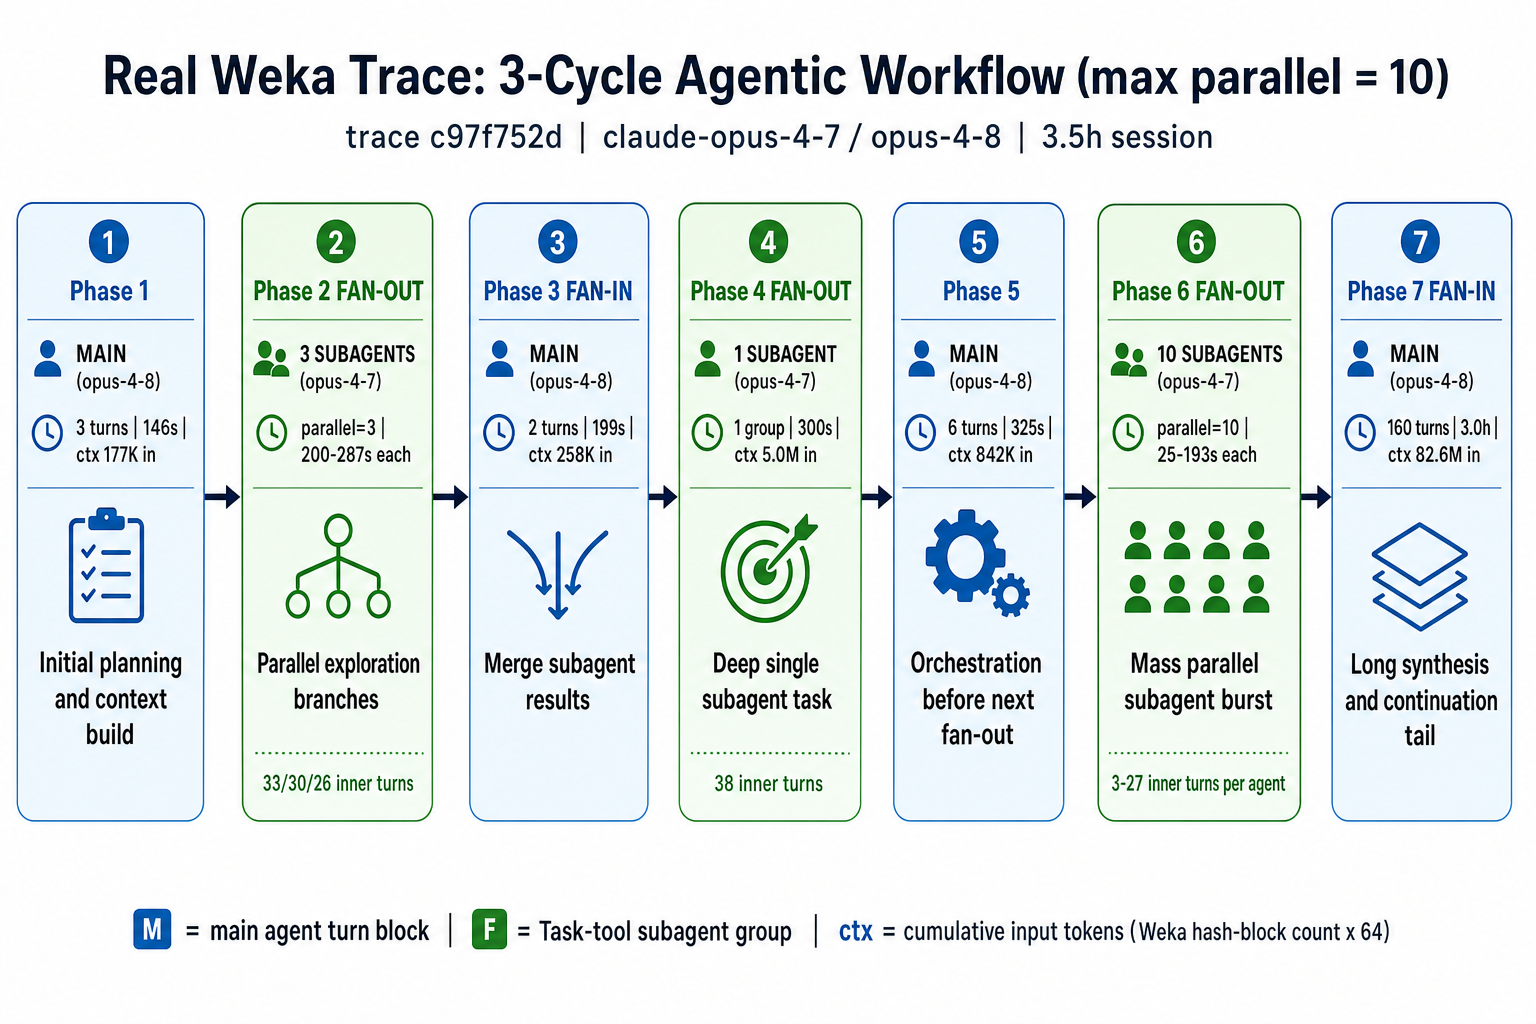
\includegraphics[width=0.98\textwidth]{fig_weka_trace_3cycle_workflow.png}
  \end{figure}
  \vspace{-0.14cm}
  \scriptsize
  Weka trace \code{c97f752d}：3 轮 fan-out/fan-in、最大并行 10、总时长 3.5h。Phase 1/3/5/7 为 main agent（opus-4-8）；Phase 2/4/6 为 Task-tool subagent group（opus-4-7）。ctx 为 Weka 输入 token 累计（hash-block $\times$ 64）；Weka 不含自然语言 prompt，主要内容按 stage 功能归纳。
\end{frame}

\begin{frame}{真实 Trace 观察 1：KV 复用主要发生在 Agent 内}
  \centering
  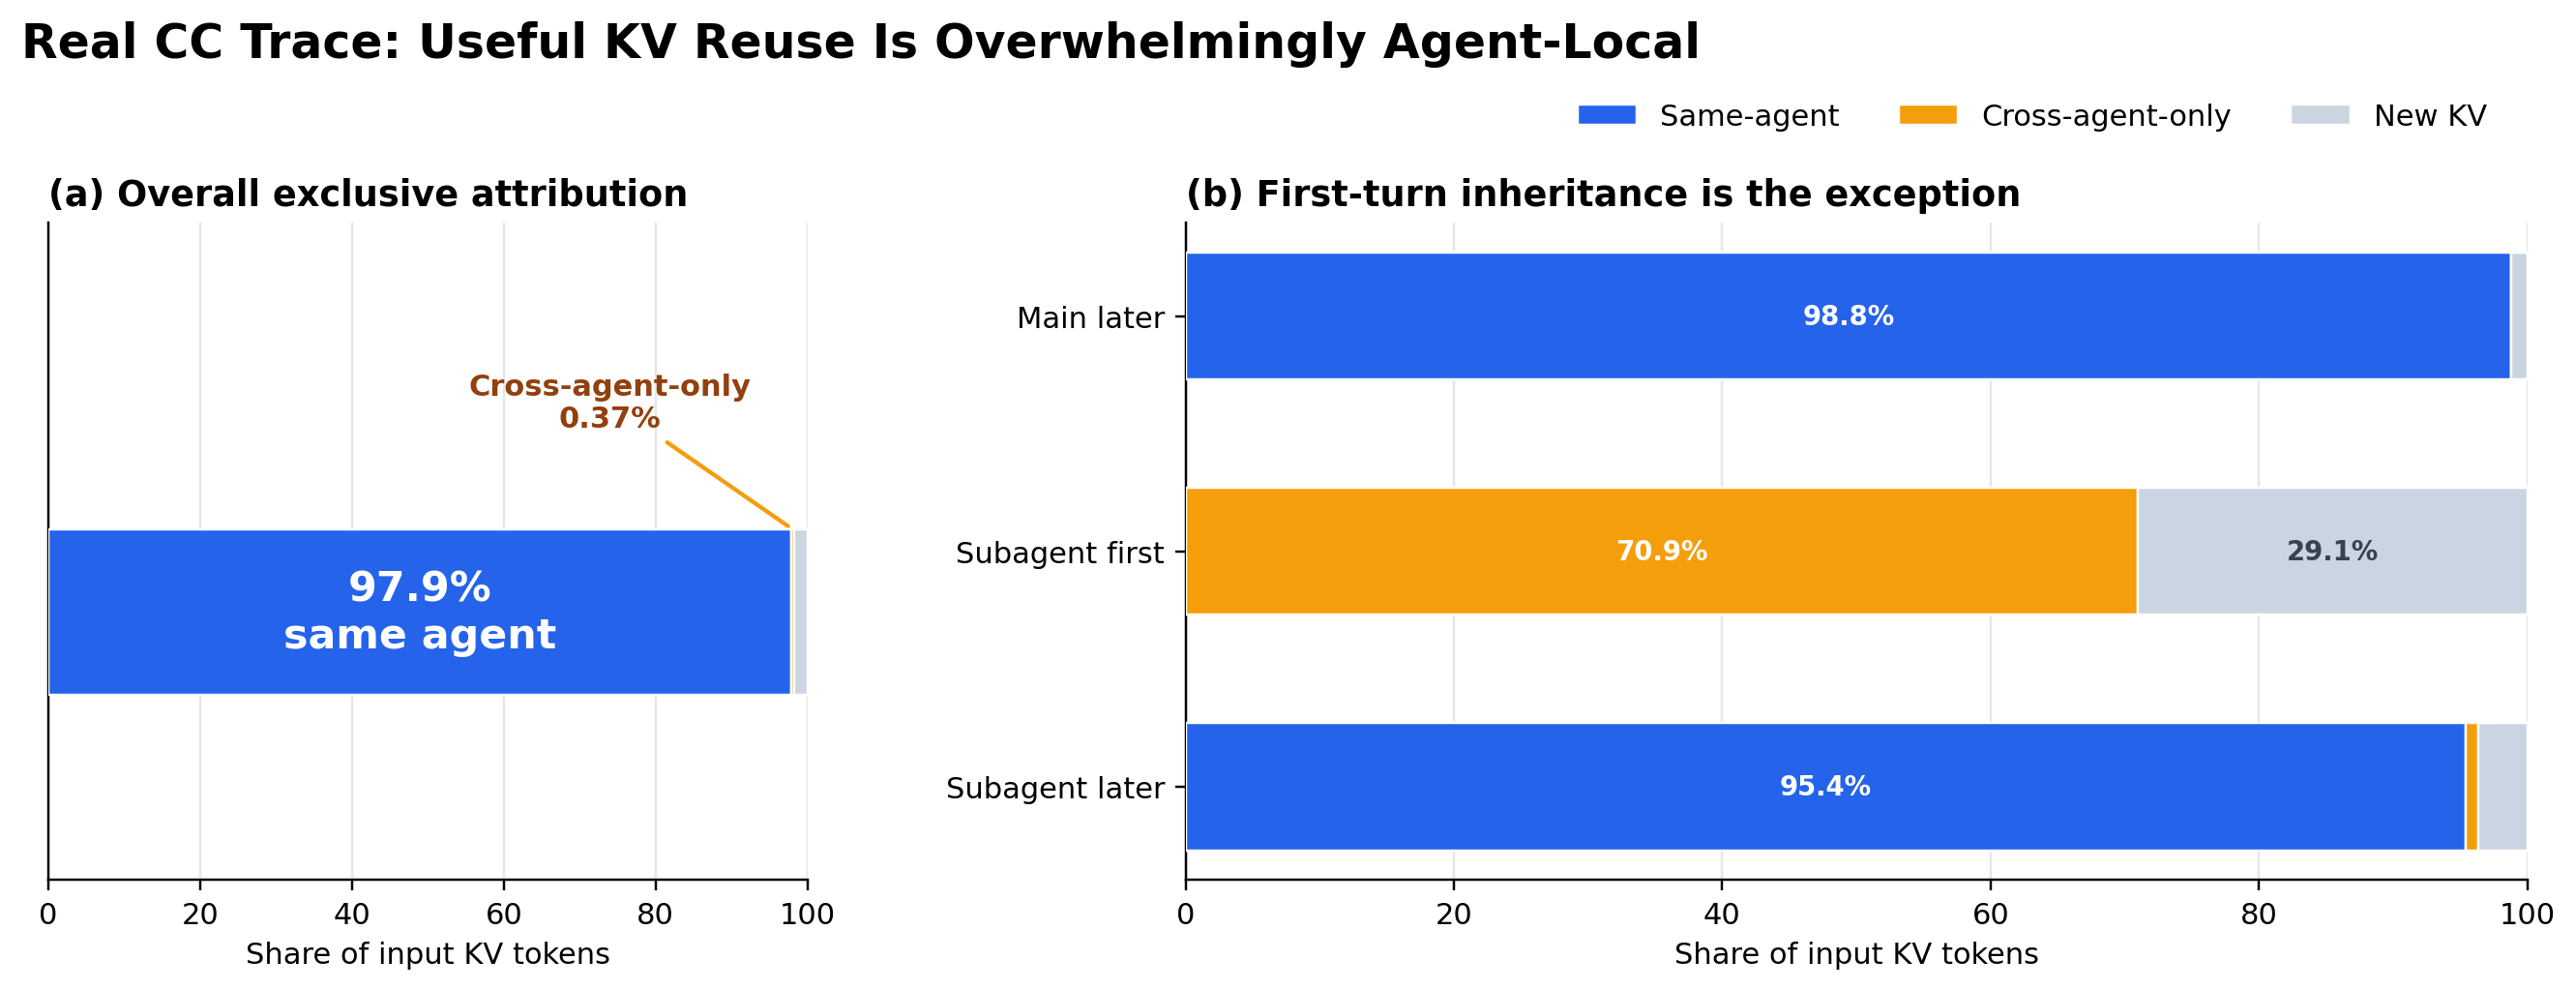
\includegraphics[width=1.02\textwidth]{fig_real_trace_kv_reuse_scope.png}

  \vspace{-0.03cm}
  \scriptsize
  393 个 workflow、98,827 条请求：按互斥 token 归因，97.90\% 来自同一 agent 历史；跨 agent 相对同-agent history 新增的可复用 KV 仅 0.37\%。Subagent first turn 的跨 agent 上下文继承是明确的局部例外。
\end{frame}

\begin{frame}{观察 2：Context Length vs. 执行时间}
  \centering
  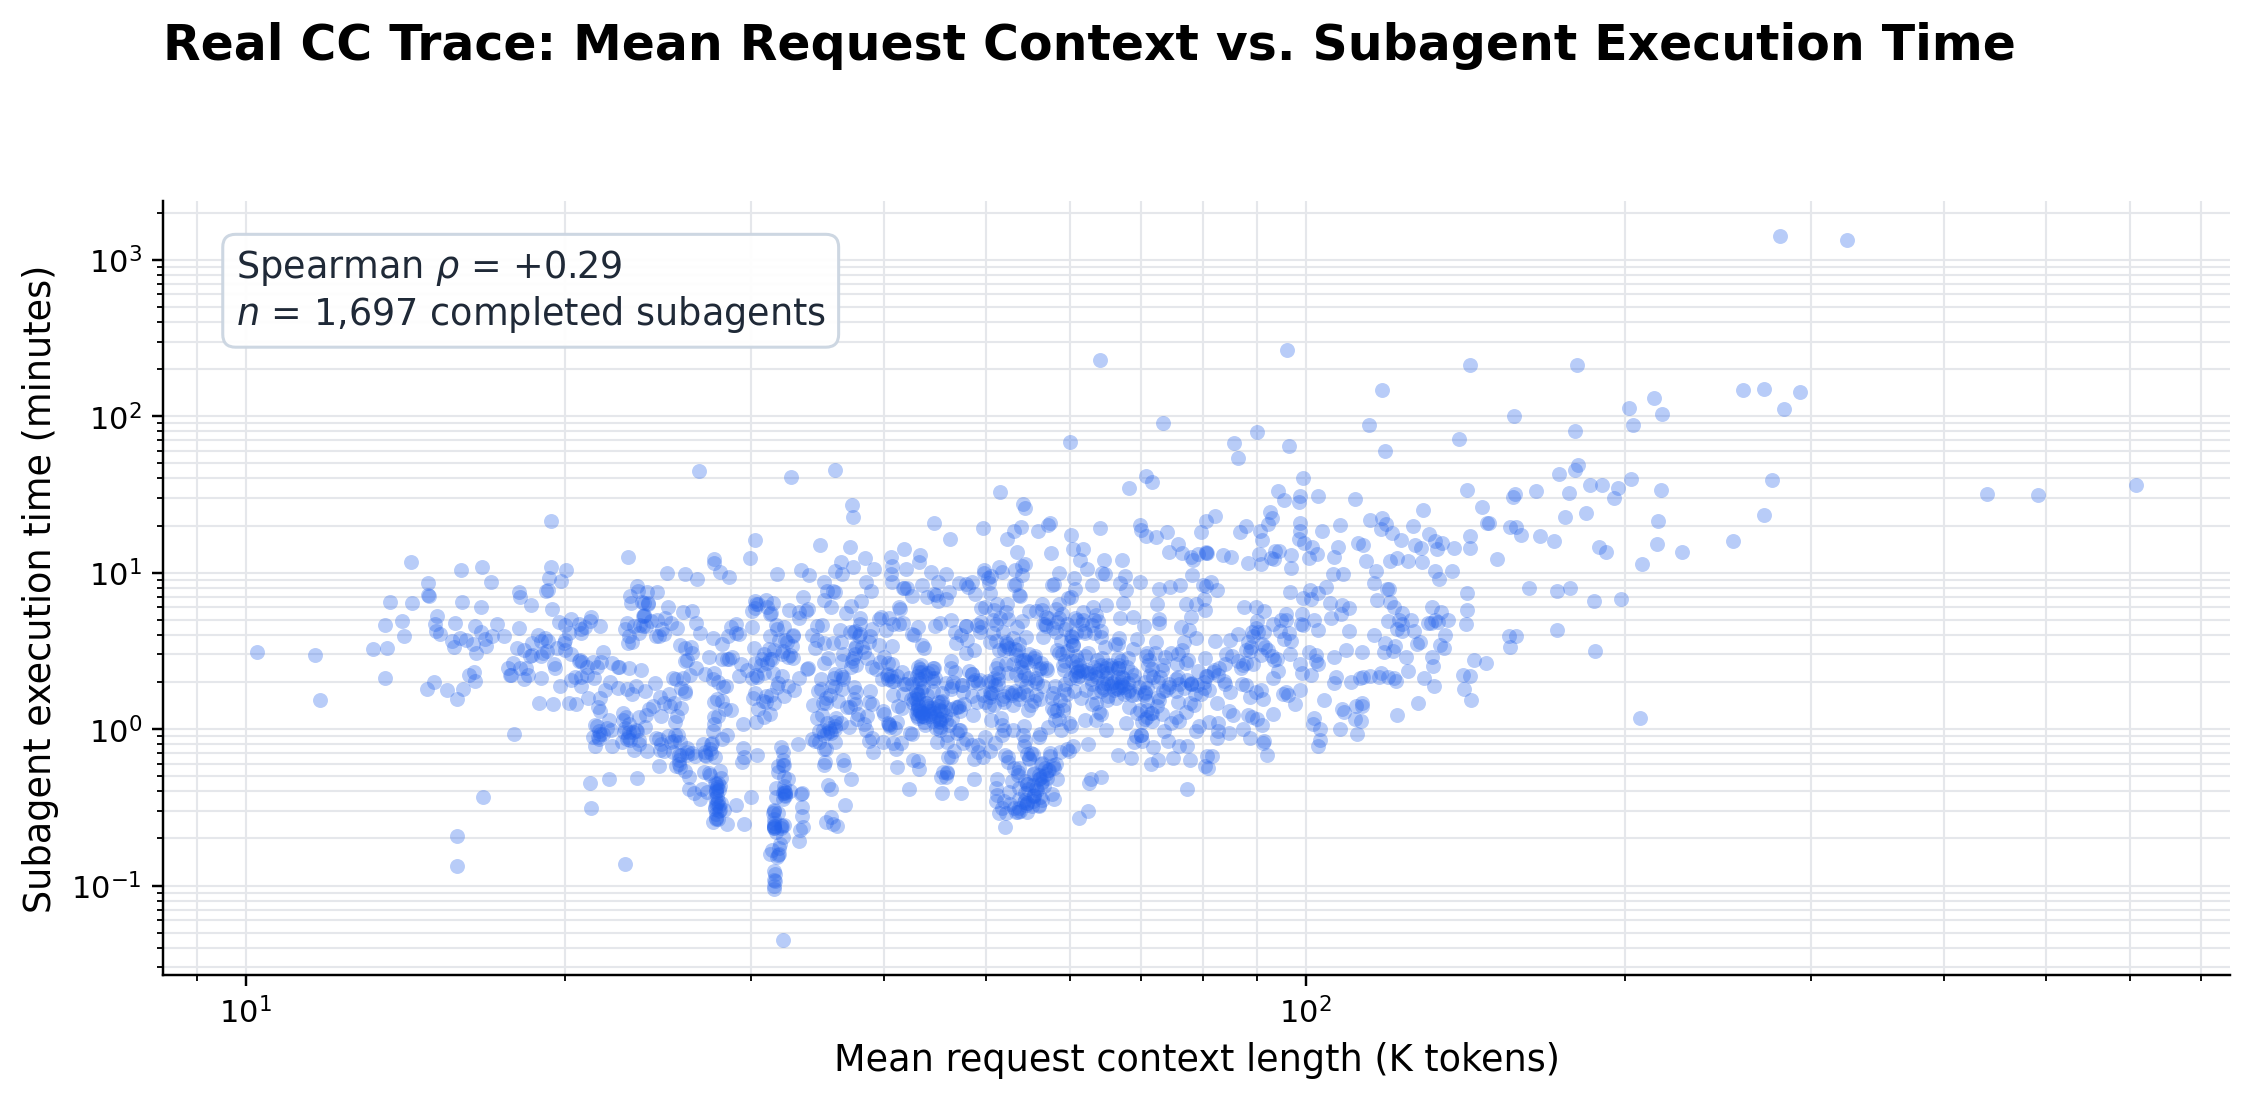
\includegraphics[width=1.02\textwidth]{fig_real_trace_context_value.png}

  \vspace{-0.03cm}
  \scriptsize
  每个点表示一个 completed subagent；context length 为该 subagent 所有请求 input length 的平均值。平均 context 与总执行时间的 Spearman $\rho=0.29$，相关性较弱，说明 context size 本身不能可靠预测 agent 会运行多久。
\end{frame}

\begin{frame}{动机实验 Setup}
  \scriptsize
  \renewcommand{\arraystretch}{1.12}
  \begin{tabular}{p{0.22\textwidth}p{0.68\textwidth}}
    \toprule
    维度 & 配置 \\
    \midrule
    平台 & SGLSim online serving；DP=8；SGLang-style Engine / Scheduler / HiCache 拓扑 \\
    模型 / workload & Qwen3-8B style metadata serving；1-3-1-3-1 agentic workflow \\
    Context pressure & 每个 subagent 约 40K tokens；main-agent 聚合上下文约 80K / 120K tokens \\
    备份策略 & no-backup baseline；仅测量 failure 对 WCT 的原始影响，不引入 AegisKV policy \\
    故障注入 & soft GPU failure；控制 target stage、agent、turn index 和 output-token offset \\
    主指标 & Workflow Completion Time (WCT)；辅以 output-token / latency exposure \\
    \midrule
    实验 1 & 8 workflow groups，max\_concurrency=24；每 workflow 注入 1 次 soft failure，扫 7 个 failure slot + no-failure baseline \\
    实验 2 & 与实验 1 共用高并发 no-failure run；统计 Critical/Non-Critical 的 workflow-level mean + 95\% CI \\
    实验 3 & 3-seed paired replay（12 staged failure case）+ 205 个 Claude Code real-trace failure position \\
    \bottomrule
  \end{tabular}

  \vspace{0.10cm}
  \footnotesize
  三组动机实验共用同一 staged workflow 与 failure-control 接口；差别在于比较维度分别为 failure position、criticality 统计分布，以及跨 seed / real trace 的 replay 稳定性。
\end{frame}

\begin{frame}{动机实验 1：故障影响取决于 Workflow 位置}
  \vspace{-0.12cm}
  \begin{figure}
    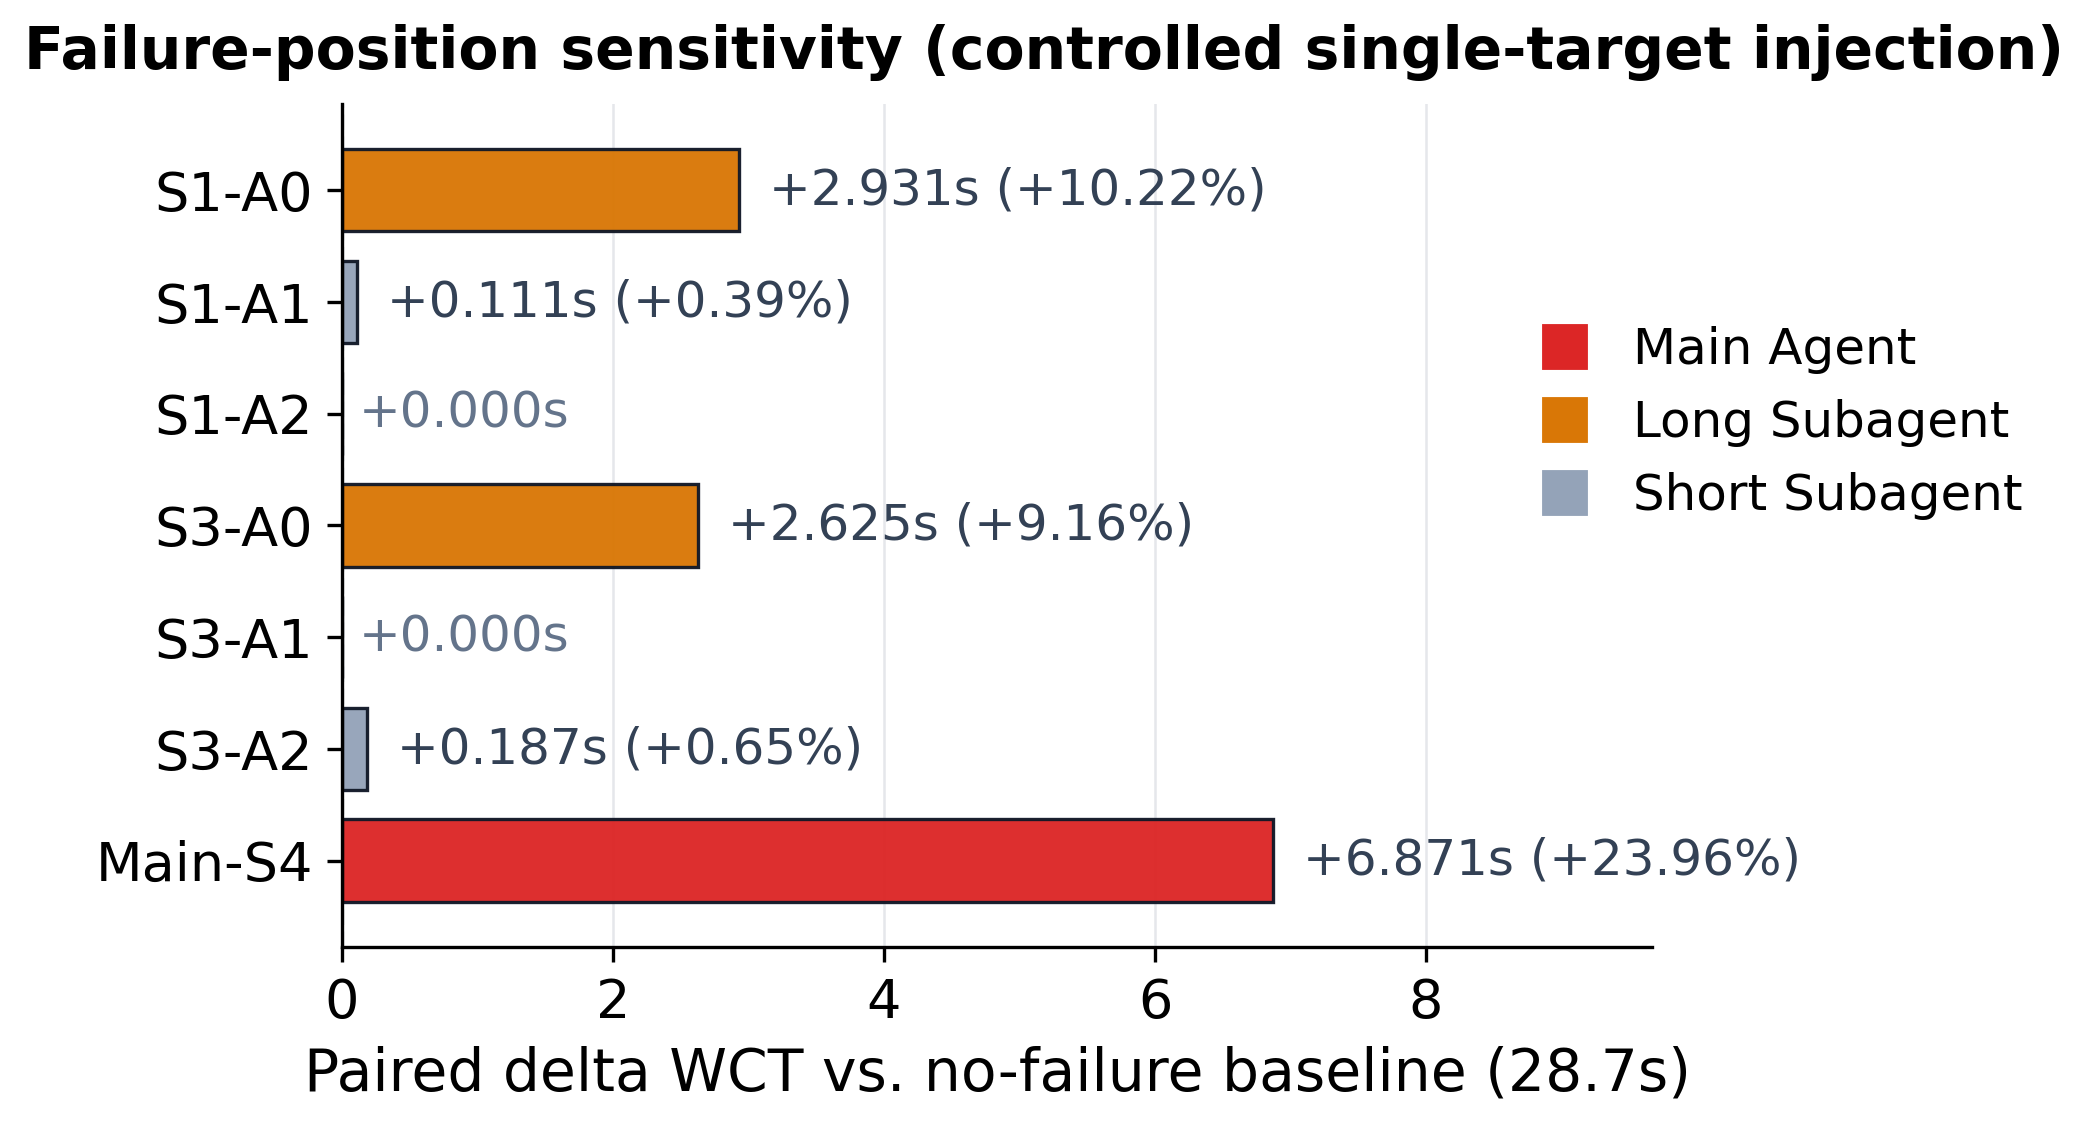
\includegraphics[width=0.50\textwidth]{fig_motivation_agent_failure_impact.png}
    \hfill
    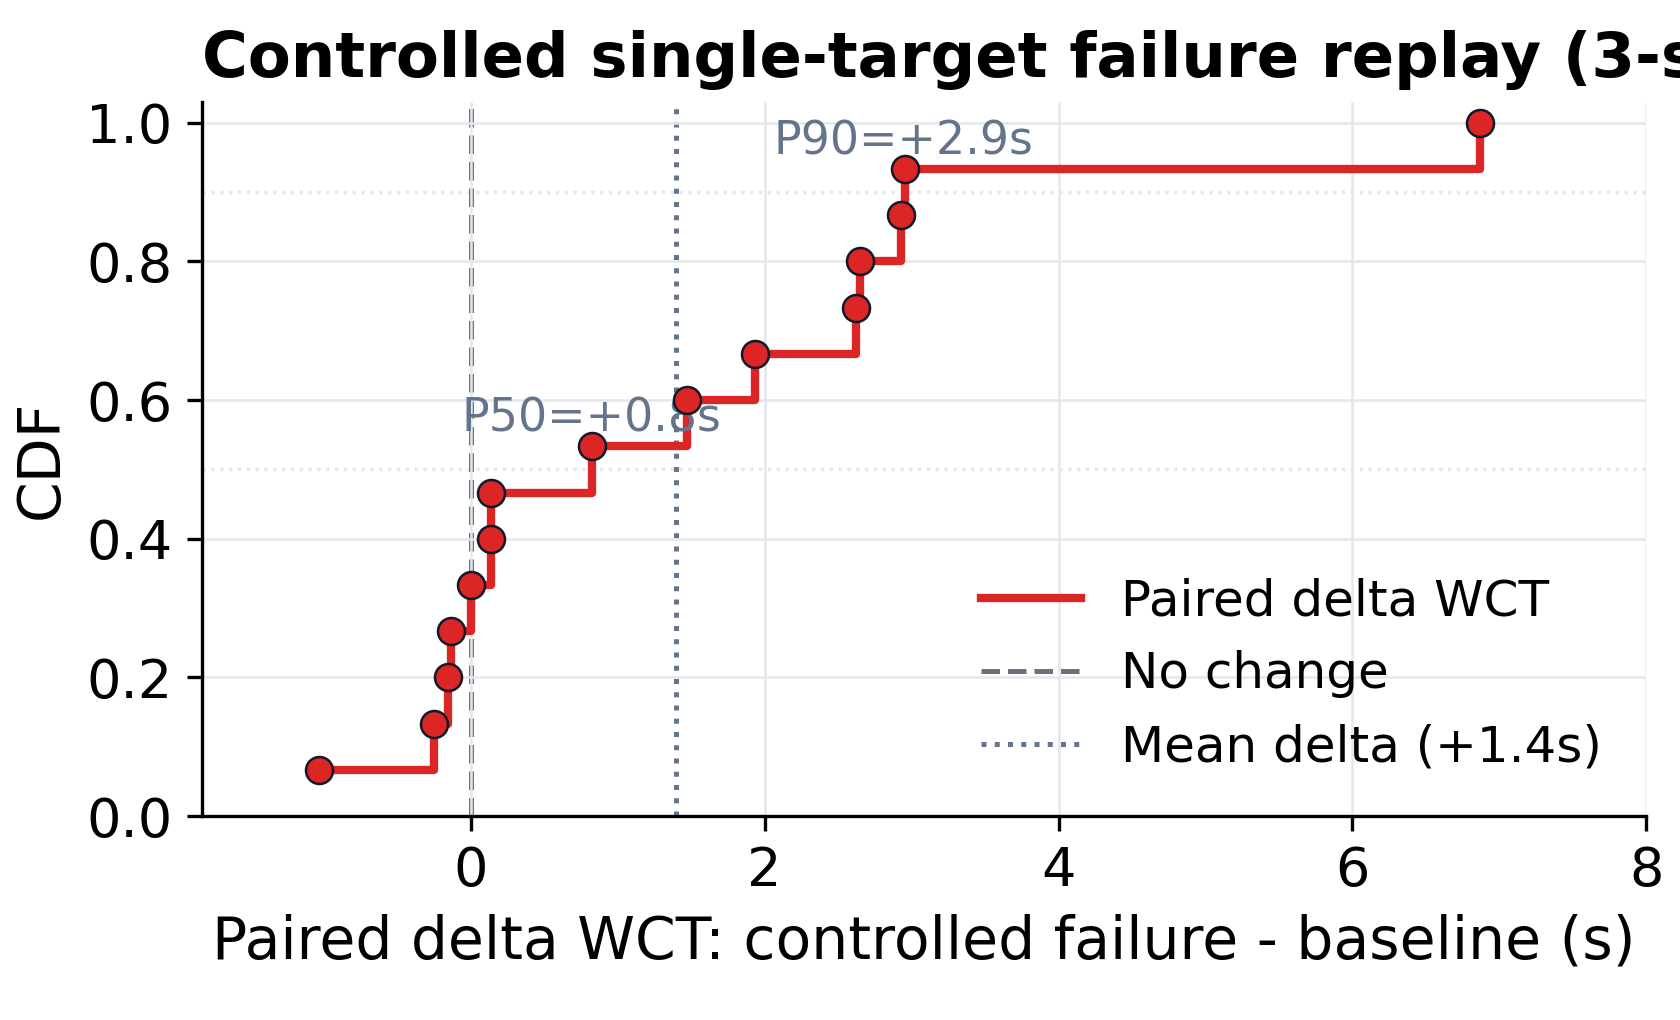
\includegraphics[width=0.48\textwidth]{fig_motivation_agent_failure_wct_cdf.png}
  \end{figure}
  \vspace{-0.18cm}
  \scriptsize
  左：7 个 failure slot 的 mean paired $\Delta$WCT（8 workflow groups，max\_concurrency=24）。右：no-failure 与全部 failure scenario 的 per-workflow WCT CDF。
\end{frame}

\begin{frame}{动机实验 2：关键性差异可被统计观察}
  \centering
  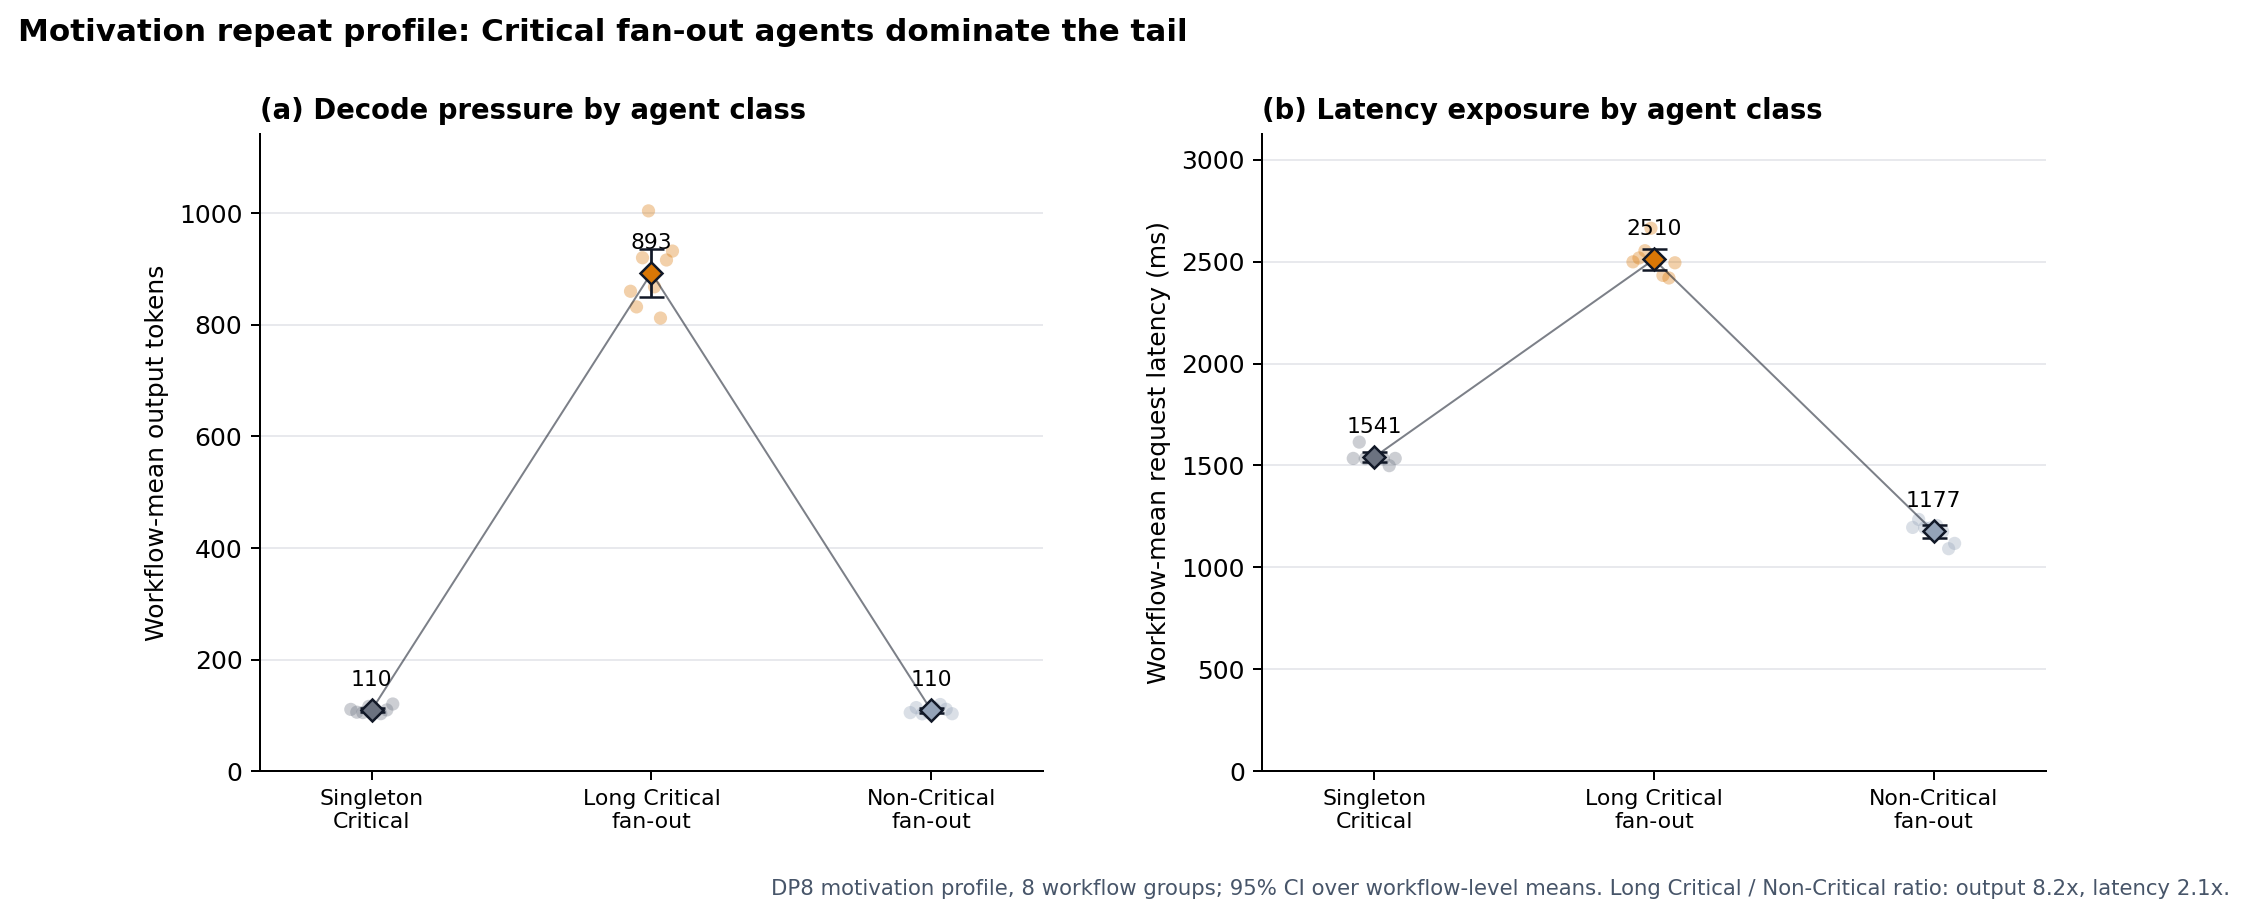
\includegraphics[width=1.03\textwidth]{fig_motivation_criticality_ci.png}

  \vspace{0.05cm}
  \footnotesize
  基于 8 个 workflow group 的 workflow-level mean 和 95\% CI。Long \Critical{} fan-out agent 的 output-token exposure 约为 \NonCritical{} fan-out agent 的 8.2$\times$，latency exposure 约为 2.1$\times$。
\end{frame}

\begin{frame}{动机实验 3：多次 Failure Replay 验证}
  \centering
  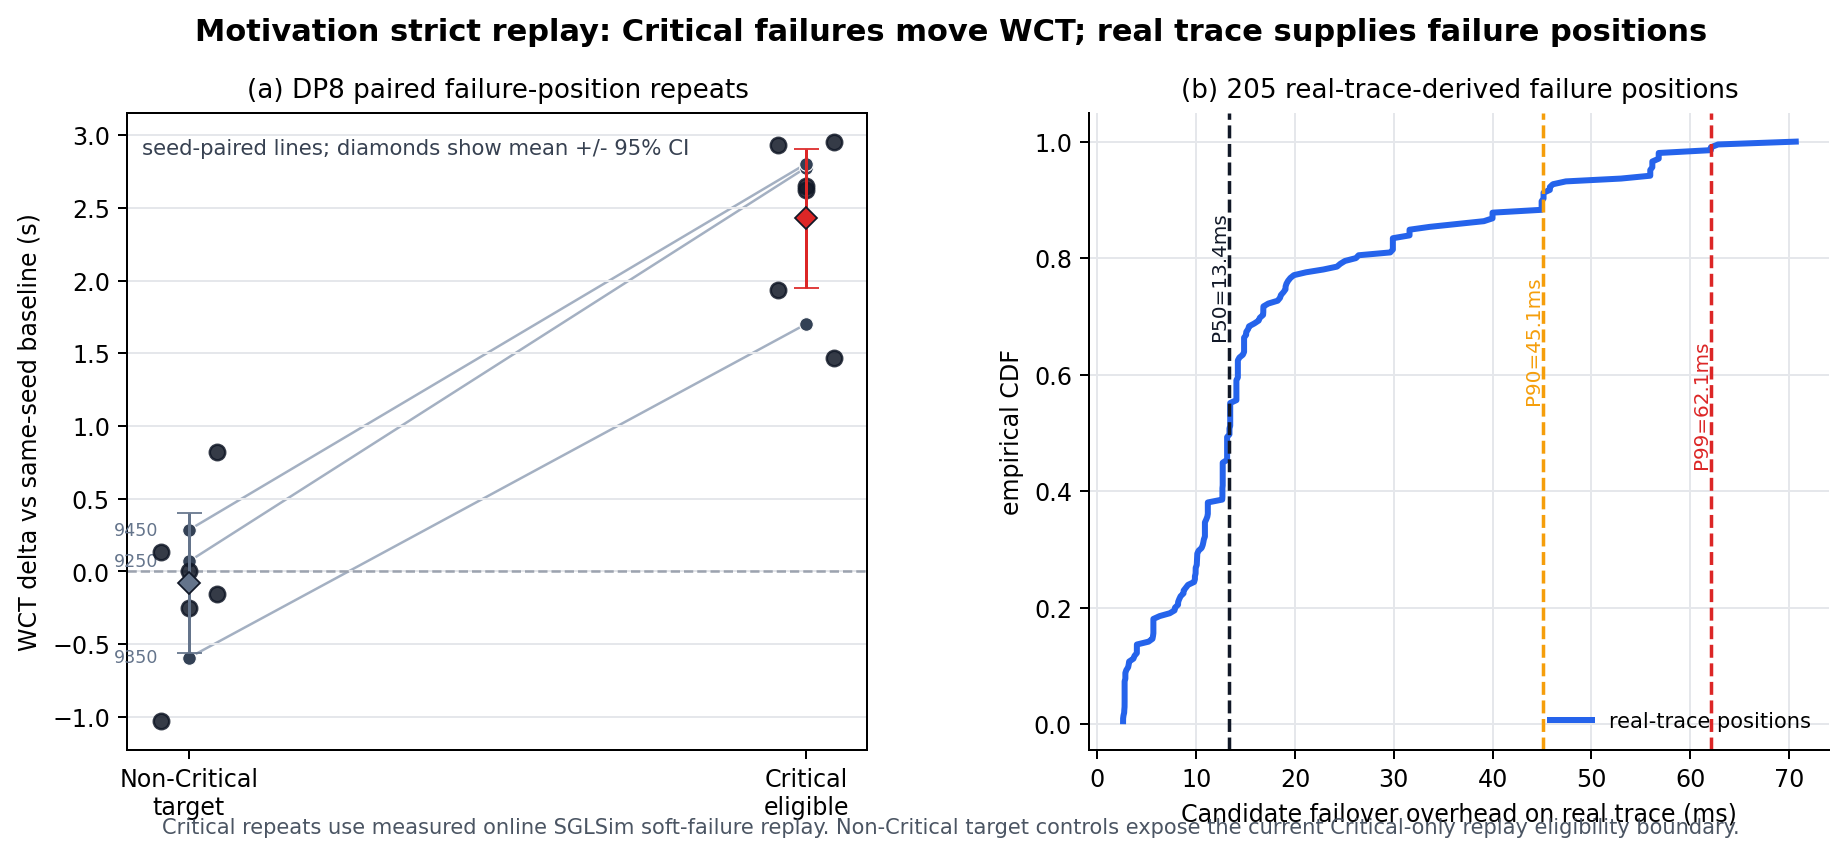
\includegraphics[width=1.03\textwidth]{fig_motivation_failure_replay_repeats.png}

  \vspace{0.05cm}
  \footnotesize
  DP8 staged workload 上的 3-seed paired replay 显示，\Critical{} soft-failure target 相对 same-seed baseline 平均增加 2.43s WCT；\NonCritical{} control positions 没有产生同等 replay overhead。右图把 205 个 Claude Code real-trace-derived candidate failure positions 接入同一套 recovery-cost 字段。
\end{frame}

%------------------------------------------------------------
\section{背景与定位}
%------------------------------------------------------------

\begin{frame}{AegisKV 基于 SGLang 的实现映射}
  \scriptsize
  \AegisKV{} 叠加在 SGLang serving substrate 上，不替换 KV manager；在 SGLang 既有 KV 生命周期上附加 workflow-aware backup 与 recovery 控制面。

  \vspace{0.06cm}
  \renewcommand{\arraystretch}{1.08}
  \begin{tabular}{
    >{\raggedright\arraybackslash}p{0.22\textwidth}
    >{\raggedright\arraybackslash}p{0.24\textwidth}
    >{\raggedright\arraybackslash}p{0.42\textwidth}
  }
    \toprule
    SGLang 机制 & AegisKV 模块 & 实现行为 \\
    \midrule
    Radix prefix cache & Workflow metadata propagation & 写入 workflow id、stage、role、turn、critical span 与 token segment \\
    HiCache write-through D2H & \HostBackup{} directory & ACK 后把 source-rank Host KV 发布为 cross-rank recoverable frontier \\
    HiCache load / H2D restore & Failure-time restore scheduler & 将 failed-rank Host KV 恢复到 retry rank，并 materialize prefix metadata \\
    DP controller / scheduler & Retry routing & 路由 retry 并在 GPUReplica / Host restore / recompute 间选最低代价 action \\
    Lock / ref / eviction state & Shared safe frontier manager & 拒绝 pending D2H、evicted Host page 与 stale ACK / epoch \\
    Prefix matching & Restore planner & 区分 device hit、Host restore 与 suffix recompute \\
    GPU KV pool / HBM budget & \GPUReplica{} + $\alpha$ partition & 在 $(1-\alpha)M_g$ inference 与 $\alpha M_g$ backup 间划分 HBM；复制 selected \Critical{} KV 到 peer GPU \\
    Cache-aware routing signals & Backup placement planner & 复用 prefix locality 与 load 信号，为 future retry 选择 peer backup rank \\
    \bottomrule
  \end{tabular}

  \vspace{0.08cm}
  \footnotesize
  Baseline 与 \AegisKV{} 都支付 fixed write-through D2H 共同成本；差别在于 retry rank 能否发现并使用 failed rank 上 ACKed Host KV，以及是否在 peer GPU 上保留 \Critical{} replica。
\end{frame}

\begin{frame}{第一篇系统只保留两个备份层级}
  \small
  \begin{columns}[T,onlytextwidth]
    \begin{column}{0.49\textwidth}
      \begin{block}{\HostBackup}
        \begin{itemize}
          \tightitems
          \item 使用 SGLang fixed write-through 路径
          \item source-rank Host KV 在 GPU failure 后存活
          \item 容量大，但 recovery 需要 H2D / cross-rank restore
          \item 贡献点：recovery directory 和 safe frontier visibility
        \end{itemize}
      \end{block}
    \end{column}
    \begin{column}{0.49\textwidth}
      \begin{block}{\GPUReplica}
        \begin{itemize}
          \tightitems
          \item selected \Critical{} KV 被复制到 peer GPU
          \item peer 健康时提供最快 recovery path
          \item 消耗 backup HBM 和 P2P/copy bandwidth
          \item 由 placement 和 alpha budget 控制
        \end{itemize}
      \end{block}
    \end{column}
  \end{columns}

  \vspace{0.12cm}
  \footnotesize
  Remote-store replication 是后续扩展；本文聚焦 Host/GPUReplica 这个能在 SGLang 与 SGLSim 上形成闭环证据的系统。
\end{frame}

%------------------------------------------------------------
\section{问题建模}
%------------------------------------------------------------

\begin{frame}{目标函数：Workflow Completion Time}
  \small
  \AegisKV{} 优化 workflow-level tail cost，而不是 request-local recovery time：

  \vspace{0.12cm}
  \[
    \min \operatorname{P99}\left(\operatorname{WCT}(w)\right),
    \qquad w \in \mathcal{W}.
  \]

  \vspace{0.10cm}
  \begin{itemize}
    \tightitems
    \item WCT 包含正常执行、failure detection、retry routing、restore 和 suffix recompute。
    \item \Critical{} 和 \NonCritical{} agent 都贡献 WCT 和 queueing。
    \item 只有 \Critical{} segments 可进入 \GPUReplica{} admission。
    \item 价值按 content 计数：Host 和 GPUReplica 覆盖同一 radix prefix 时只记一次收益。
  \end{itemize}
\end{frame}

\begin{frame}{Backup / Inference HBM 划分}
  \small
  对 GPU $g$，\AegisKV{} 把可控 HBM budget $M_g$ 划分为：

  \vspace{0.10cm}
  \[
    M_{\mathrm{Backup}}(g,t) = \alpha_{g,t} M_g,
    \qquad
    M_{\mathrm{Inference}}(g,t) = (1-\alpha_{g,t})M_g .
  \]

  \vspace{0.10cm}
  \begin{block}{核心张力}
    更大的 $\alpha$ 能保护更多 \Critical{} KV，降低故障恢复代价；更小的 $\alpha$ 给 active KV、prefix cache、admission 和 normal serving throughput 留出更多 HBM。
  \end{block}

  \vspace{0.10cm}
  \footnotesize
  $\boldsymbol{\alpha}_t=(\alpha_{1,t},\ldots,\alpha_{G,t})$ 是当前全局 allocation state；controller 的 action 是下一页中的小步长 $\Delta\boldsymbol{\alpha}_t$。Reward 只在 workflow level 计算一次，因为一个 workflow 会跨多个 ranks。
\end{frame}

\begin{frame}{MDP 控制器}
  \small
  在线控制器可以写成 MDP：

  \vspace{0.04cm}
  \[
    (\mathcal{S},\mathcal{A},\mathcal{P},\mathcal{R},\gamma),
    \qquad
    J(\pi)=\mathbb{E}_{\pi}\left[\sum_{t=0}^{\infty}\gamma^t r_t\right].
  \]

  \vspace{-0.08cm}
  \scriptsize
  下表是状态向量
  $s_t=(h_t,k_t,e_t,L_t,v_t,\alpha_t,p_t)\in\mathcal{S}$ 的 7 个分量；不是 MDP tuple 里的全部符号。

  \vspace{0.04cm}
  \renewcommand{\arraystretch}{1.10}
  \begin{tabular}{p{0.15\textwidth}p{0.72\textwidth}}
    \toprule
    状态分量 & AegisKV 中的观测含义 \\
    \midrule
    $h_t$ & \Critical{} request pressure \\
    $k_t$ & inference partition 中的 critical KV / prefix hit rate \\
    $e_t$ & candidate retry tokens 上的 effective backup coverage \\
    $L_t$ & critical context length 或 token-length pressure \\
    $v_t$ & workflow SLO violation fraction \\
    $\alpha_t$ & 当前 backup/inference allocation ratio；action 是 $\Delta\alpha_t$ \\
    $p_t$ & normalized P99 WCT \\
    \bottomrule
  \end{tabular}

  \vspace{0.08cm}
  \footnotesize
  Action 是对 $\alpha$ 的小步长 clipped update；reward 综合 SLO satisfaction、P99 WCT violation 和 normal-path overhead。
\end{frame}

\begin{frame}{Segment 放置与恢复动作}
  \small
  令 $\mathcal{N}_t$ 表示可见 radix segments，$\mathcal{C}_t$ 表示 \Critical{} segments：

  \vspace{0.05cm}
  \[
    \mathcal{C}_t =
    \{ n\in\mathcal{N}_t \mid \operatorname{critical}(n)=1 \},
    \qquad
    x_{n,t}=0\quad\forall n\notin\mathcal{C}_t .
  \]

  \vspace{0.08cm}
  故障时，每个 retry request 选择最低代价的 safe action：

  \vspace{0.05cm}
  \[
    \operatorname{cost}(n) =
    \min\{
      C_{\mathrm{gpu\_replica}}(n),
      C_{\mathrm{host}}(n),
      C_{\mathrm{recompute}}(n)
    \}.
  \]

  \vspace{0.08cm}
  \begin{itemize}
    \tightitems
    \item pending D2H 或 peer copy 在 ACK 前不是 safe frontier。
    \item Host eviction 和 peer invalidation 会撤销对应 frontier。
    \item 若 restore queue 比 recompute 更慢，短 suffix 可以选择重算。
  \end{itemize}
\end{frame}

%------------------------------------------------------------
\section{系统设计}
%------------------------------------------------------------

\begin{frame}[t]{系统总览：场景、部署与 AegisKV 模块}
  \vspace{-0.28cm}
  \centering
  \resizebox{0.99\textwidth}{!}{%
  \begin{tikzpicture}[
    font=\sffamily\footnotesize,
    >=Latex,
    flow/.style={draw=AegisLine, line width=0.72pt, -{Latex[length=2.0mm]}},
    softflow/.style={draw=AegisLine, line width=0.58pt, dashed, -{Latex[length=1.8mm]}},
    panel/.style={draw=AegisLine, fill=BackgroundLight, rounded corners=3pt, line width=0.76pt},
    card/.style={draw=AegisLine, fill=white, rounded corners=2pt, line width=0.68pt, align=center},
    module/.style={card, minimum height=0.48cm, inner xsep=4pt, font=\sffamily\scriptsize},
    nodecard/.style={draw=AegisLine, fill=white, rounded corners=2pt, line width=0.76pt},
    stage/.style={card, fill=AegisBlueLight, draw=AegisBlue, minimum width=1.32cm, minimum height=0.58cm, font=\sffamily\scriptsize},
    hbm/.style={card, fill=AegisOrangeLight, draw=AegisOrange, minimum height=0.38cm, font=\sffamily\scriptsize},
    host/.style={card, fill=AegisHost, draw=AegisLine, minimum height=0.38cm, font=\sffamily\scriptsize},
    title/.style={font=\sffamily\bfseries\small, anchor=west},
    sub/.style={font=\sffamily\scriptsize, text=TextSecondary}
  ]
    \node[panel, minimum width=4.15cm, minimum height=1.02cm, anchor=north west] (entry) at (0.12,6.34) {};
    \node[title] at ($(entry.north west)+(0.22,-0.25)$) {Agentic serving entry};
    \node[module, minimum width=1.34cm] (request) at ($(entry.north west)+(0.84,-0.70)$) {Requests};
    \node[module, minimum width=1.56cm, fill=AegisBlueLight, draw=AegisBlue] (router) at ($(entry.north west)+(2.90,-0.70)$) {Router / Engine};
    \draw[flow] (request.east) -- (router.west);

    \node[panel, minimum width=6.86cm, minimum height=1.02cm, anchor=north west] (control) at (4.86,6.34) {};
    \node[title] at ($(control.north west)+(0.22,-0.25)$) {AegisKV software design};
    \node[module, minimum width=1.36cm, fill=AegisPurpleLight, draw=AegisPurple] (meta) at ($(control.north west)+(1.06,-0.70)$) {Metadata};
    \node[module, minimum width=1.50cm, fill=AegisOrangeLight, draw=AegisOrange] (hostdir) at ($(control.north west)+(3.25,-0.70)$) {HostBackup};
    \node[module, minimum width=1.50cm, fill=AegisGreenLight, draw=AegisGreen] (replica) at ($(control.north west)+(5.52,-0.70)$) {GPUReplica};
    \draw[flow] (router.east) -- (control.west);

    \node[panel, minimum width=11.60cm, minimum height=4.38cm, anchor=north west] (deploy) at (0.12,5.04) {};
    \node[title] at ($(deploy.north west)+(0.26,-0.28)$) {Multi-node LLM deployment: DP replicas + PP stages};

    \node[nodecard, minimum width=4.72cm, minimum height=2.28cm, anchor=north west] (n0) at (0.72,4.38) {};
    \node[title] at ($(n0.north west)+(0.22,-0.25)$) {Node 0 / DP 0};
    \node[sub, anchor=west] at ($(n0.north west)+(0.22,-0.52)$) {failure target};
    \draw[draw=red!70!black, line width=1.05pt] ($(n0.north east)+(-0.46,-0.22)$) -- ($(n0.north east)+(-0.18,-0.50)$);
    \draw[draw=red!70!black, line width=1.05pt] ($(n0.north east)+(-0.18,-0.22)$) -- ($(n0.north east)+(-0.46,-0.50)$);
    \node[stage] (n0pp0) at ($(n0.north west)+(1.30,-1.02)$) {PP0\\GPU0};
    \node[stage] (n0pp1) at ($(n0.north west)+(3.18,-1.02)$) {PP1\\GPU1};
    \draw[flow] (n0pp0.east) -- (n0pp1.west);
    \node[hbm, minimum width=3.96cm] (n0hbm) at ($(n0.north west)+(2.36,-1.62)$) {GPU HBM: active KV};
    \node[host, minimum width=3.96cm] (n0cpu) at ($(n0.north west)+(2.36,-2.08)$) {CPU KV pages};

    \node[nodecard, minimum width=4.72cm, minimum height=2.28cm, anchor=north west] (n1) at (6.46,4.38) {};
    \node[title] at ($(n1.north west)+(0.22,-0.25)$) {Node 1 / DP 1};
    \node[sub, anchor=west] at ($(n1.north west)+(0.22,-0.52)$) {healthy peer};
    \node[stage] (n1pp0) at ($(n1.north west)+(1.30,-1.02)$) {PP0\\GPU2};
    \node[stage] (n1pp1) at ($(n1.north west)+(3.18,-1.02)$) {PP1\\GPU3};
    \draw[flow] (n1pp0.east) -- (n1pp1.west);
    \node[hbm, minimum width=3.96cm, fill=AegisGreenLight, draw=AegisGreen] (n1hbm) at ($(n1.north west)+(2.36,-1.62)$) {GPU HBM: replica slot};
    \node[host, minimum width=3.96cm] (n1cpu) at ($(n1.north west)+(2.36,-2.08)$) {CPU KV pages};

    \draw[flow, draw=AegisGreen] (n0hbm.east) -- (n1hbm.west);

    \node[host, minimum width=10.52cm, minimum height=0.76cm, anchor=north west] (shared) at (0.72,1.58) {};
    \node[font=\sffamily\bfseries\scriptsize] at ($(shared.north)+(0,-0.24)$) {Shared Host Memory / HostBackup namespace};
    \node[sub] at ($(shared.south)+(0,0.22)$) {ACKed KV pages, recovery directory, safe frontier};
    \draw[flow, draw=AegisOrange] (n0cpu.south) -- ++(0,-0.26) -- (shared.north -| n0cpu.south);
    \draw[flow, draw=AegisOrange] (n1cpu.south) -- ++(0,-0.26) -- (shared.north -| n1cpu.south);

  \end{tikzpicture}}
\end{frame}

\begin{frame}{系统组件}
  \small
  \begin{enumerate}
    \tightitems
    \item \textbf{Workflow metadata propagation}：把 workflow id、stage、agent role、turn、lifecycle、failure target 和 token span 写入 request/radix metadata。
    \item \textbf{HostBackup recovery directory}：ACKed write-through Host KV 发布为 cross-rank recoverable frontier。
    \item \textbf{Backup placement planner}：评估 workflow value、recompute cost、resource pressure 和 peer locality。
    \item \textbf{GPUReplica manager}：在 $\alpha$ budget 下把 selected \Critical{} segments 放入 peer backup HBM。
    \item \textbf{Shared safe frontier manager}：对 Host 和 GPUReplica 覆盖的同一 content prefix 做去重。
    \item \textbf{Failure-time restore scheduler}：为 retry 选择 GPUReplica、Host restore 或 recompute。
  \end{enumerate}
\end{frame}

\begin{frame}{HostBackup 恢复目录}
  \small
  \HostBackup{} 不是 failed GPU 上的额外副本，而是 fixed write-through 产生并在 ACK 后可见的 source-worker Host KV。

  \vspace{0.12cm}
  \scriptsize
  \renewcommand{\arraystretch}{1.10}
  \begin{tabular}{p{0.24\textwidth}p{0.58\textwidth}}
    \toprule
    字段 & 作用 \\
    \midrule
    source DP rank & 标识 Host KV 存活的 failed/source rank \\
    radix key / token span & 把 retry prefix 映射到 recoverable content \\
    host handle & 定位 Host-resident KV pages \\
    ACK epoch & 拒绝 pending 或 stale copy \\
    eviction generation & Host eviction 后撤销 frontier \\
    restore statistics & 记录 H2D/cross-rank restore 和 suffix replay \\
    \bottomrule
  \end{tabular}

  \vspace{0.12cm}
  \footnotesize
  Baseline 也执行 write-through D2H，但没有 cross-rank directory，因此 retry 只能使用 ordinary prefix cache 或 recompute。
\end{frame}

\begin{frame}{GPUReplica 放置策略}
  \small
  \GPUReplica{} 把 selected \Critical{} KV 保护在健康 peer DP rank 上。Peer selection 复用 cache-aware routing 信号，但目标是未来 recovery：

  \vspace{0.10cm}
  \[
    \operatorname{score}(g)
    =
    \beta_{\mathrm{hit}}H_g
    -
    \beta_{\mathrm{load}}L_g
    -
    \beta_{\mathrm{mem}}P_g
    -
    \beta_{\mathrm{copy}}Q_g .
  \]

  \begin{itemize}
    \tightitems
    \item $H_g$：prefix locality 以及与现有 backup frontier 的 overlap。
    \item $L_g$：serving load 和 retry queue pressure。
    \item $P_g$：$\alpha_g$ 下的 backup partition pressure。
    \item $Q_g$：P2P/copy queue pressure 和预计 actuation cost。
  \end{itemize}
\end{frame}

\begin{frame}{Shared Safe Frontier 去重}
  \small
  Host 和 GPUReplica 可能覆盖同一段 radix prefix。若把二者作为独立收益，会夸大保护价值并浪费 backup budget。

  \vspace{0.10cm}
  \begin{block}{Content-level accounting}
    \AegisKV{} 只记录一个 safe content frontier，并附带多个 recovery choices：
    \[
      \begin{aligned}
      \mathrm{choices}(p)=\{&
        \GPUReplica(\mathrm{peer}),\ \HostBackup(\mathrm{source}),\\
        &\mathrm{recompute\_suffix}\}.
      \end{aligned}
    \]
  \end{block}

  \vspace{0.10cm}
  \begin{itemize}
    \tightitems
    \item 只有 Host 或 peer ACK 后，frontier 才能前移。
    \item Eviction 或 invalidation 只撤销对应 choice。
    \item Retry scheduler 根据实时 queue 选择最低代价的合法 choice。
  \end{itemize}
\end{frame}

\begin{frame}{故障时 Retry 路径}
  \small
  \begin{enumerate}
    \tightitems
    \item 检测 failed source DP rank，并定位受影响的 workflow requests。
    \item 查询 safe frontier registry，找到最深 recoverable prefix。
    \item 估计 peer-GPU hit/restore、Host H2D restore 和 suffix recompute。
    \item 把 retry 路由到 frontier 与 queue state 兼容的健康 rank。
    \item Materialize restored prefix metadata，并 replay missing suffix。
    \item 记录 WCT、recovery action、restored tokens、recompute tokens 和 overhead。
  \end{enumerate}

  \vspace{0.14cm}
  \begin{block}{正确性不变量}
    \AegisKV{} 不使用 pending copy、evicted Host page，或 ACK/epoch 已经不匹配的 peer replica。
  \end{block}
\end{frame}

%------------------------------------------------------------
\section{实现与实验方法}
%------------------------------------------------------------

\begin{frame}{实现边界}
  \small
  \begin{columns}[T,onlytextwidth]
    \begin{column}{0.49\textwidth}
      \begin{block}{SGLSim online path}
        \begin{itemize}
          \tightitems
          \item 真实 HTTP server 和 async client loop
          \item SGLang-like Engine、DP controller、Scheduler topology
          \item Metadata KV pool、radix、HiCache 和 pipeline timing
          \item Aegis workflow metadata、policy、failure replay 和 recovery accounting
        \end{itemize}
      \end{block}
    \end{column}
    \begin{column}{0.49\textwidth}
      \begin{block}{SGLang anchors}
        \begin{itemize}
          \tightitems
          \item no-HiCache fa3 base-serving parity
          \item physical Host H2D 与 peer P2P copy anchors
          \item strict recovery matrix 和 timing calibration
          \item SGLSim 作为 scale-up online experiment engine
        \end{itemize}
      \end{block}
    \end{column}
  \end{columns}

  \vspace{0.10cm}
  \footnotesize
  SGLSim 唯一有意替换的是 GPU forward latency prediction；scheduler、metadata、cache 和 request lifecycle 仍按 SGLang-style path 对齐。
\end{frame}

\begin{frame}{Workload 与故障注入}
  \scriptsize
  \renewcommand{\arraystretch}{1.12}
  \begin{tabular}{p{0.25\textwidth}p{0.62\textwidth}}
    \toprule
    维度 & 配置 \\
    \midrule
    模型 / 拓扑 & Qwen3-8B style metadata serving；DP=8 online SGLSim；SGLang anchors 用于 calibration \\
    Workflow & 1-3-1-3-1 agentic workflow；1 个 main-agent session；两轮 fan-out \\
    Context pressure & subagents 约 40K tokens；main-agent aggregation 接近 80K 和 120K tokens \\
    Load regimes & lite、base、high、stress、100K-context staged workloads \\
    Real trace & Claude Code：96 workflows / 205 rows；Weka \code{c97f752d}：1 workflow / 352 rows（181 parallel subagent rows，max fan-out 10） \\
    Failure control & target stage、target agent、turn index、output-token offset 和 replay count \\
    Metrics & WCT、P90/P99 latency、restore tokens、recompute tokens、recovery action、alpha、HBM pressure \\
    \bottomrule
  \end{tabular}
\end{frame}

\begin{frame}{评估问题}
  \scriptsize
  \renewcommand{\arraystretch}{1.12}
  \begin{tabular}{
    >{\raggedright\arraybackslash}p{0.12\textwidth}
    >{\raggedright\arraybackslash}p{0.43\textwidth}
    >{\raggedright\arraybackslash}p{0.32\textwidth}
  }
    \toprule
    RQ & 问题 & 证据 \\
    \midrule
    RQ1 & \Critical{} failures 是否比普通 fan-out failures 更影响 WCT？ & failure-impact curve、criticality CI、replay repeats \\
    RQ2 & 哪种 backup policy 同时改善 WCT 和 recovery overhead？ & HostBackup、GPUReplica、AegisKV、no-backup policy matrix \\
    RQ3 & Backup HBM ratio $\alpha$ 如何随 load 和 failure pressure 改变？ & measured alpha sweep 与 calibrated tradeoff \\
    RQ4 & MDP alpha policy 是否进入 online serving path？ & online alpha runs 与 row-by-row selector replay \\
    RQ5 & 真实 agentic traces 是否能走同一条 workflow-aware path？ & Claude Code trace characterization、Weka \code{c97f752d} parallel-subagent replay、selector checks \\
    RQ6 & 哪些 AegisKV components 关键？ & 11-variant ablation matrix \\
    RQ7 & SGLSim 是否有真实系统测量锚点？ & SGLang/SGLSim parity 与 recovery calibration \\
    \bottomrule
  \end{tabular}
\end{frame}

%------------------------------------------------------------
\section{实验结果}
%------------------------------------------------------------

\begin{frame}{RQ2：备份策略对比}
  \centering
  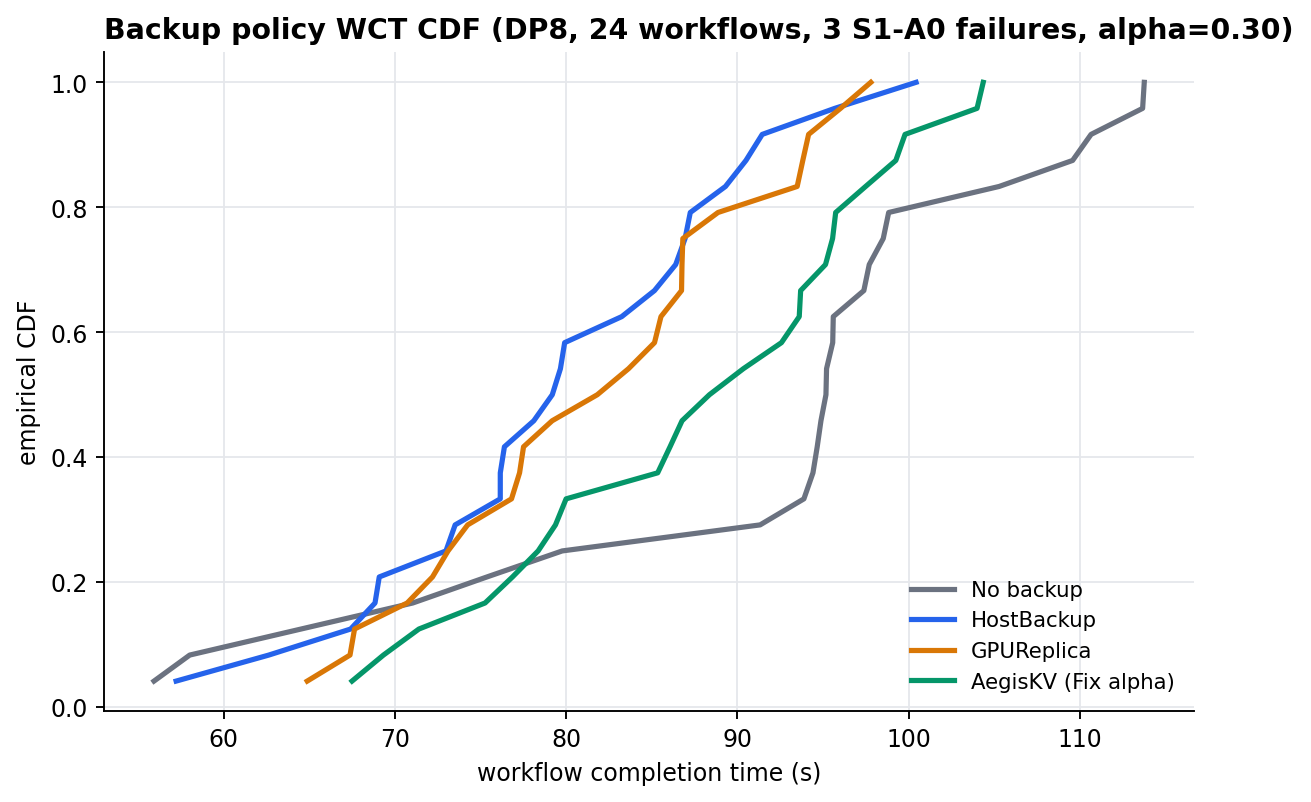
\includegraphics[width=1.04\textwidth]{fig_backup_policy_comparison.png}

  \vspace{0.06cm}
  \footnotesize
  Policy matrix 覆盖 no-backup、HostBackup、GPUReplica 和 AegisKV，包含 lite、stress、100K workloads 以及 soft / hard-restart failure timings。Per-workflow WCT 与 per-replay overhead ECDF 保留 tail behavior，而不是只报告 mean bar。
\end{frame}

\begin{frame}{RQ3：Alpha 资源权衡}
  \centering
  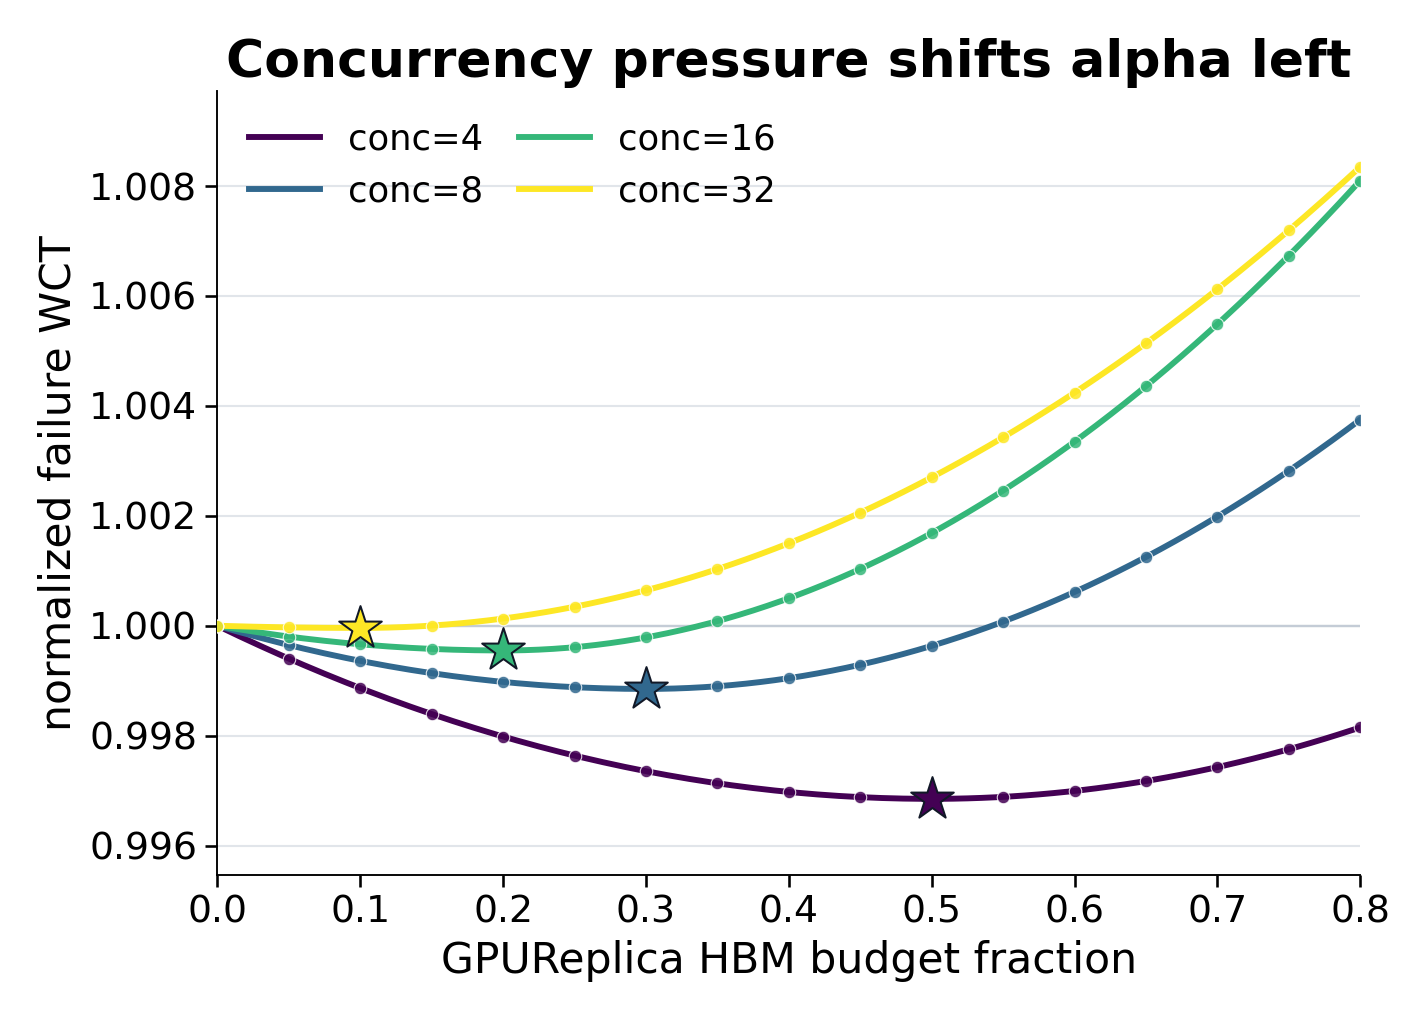
\includegraphics[width=0.98\textwidth]{fig_gpu_replica_alpha_tradeoff_concurrency.png}

  \vspace{0.04cm}
  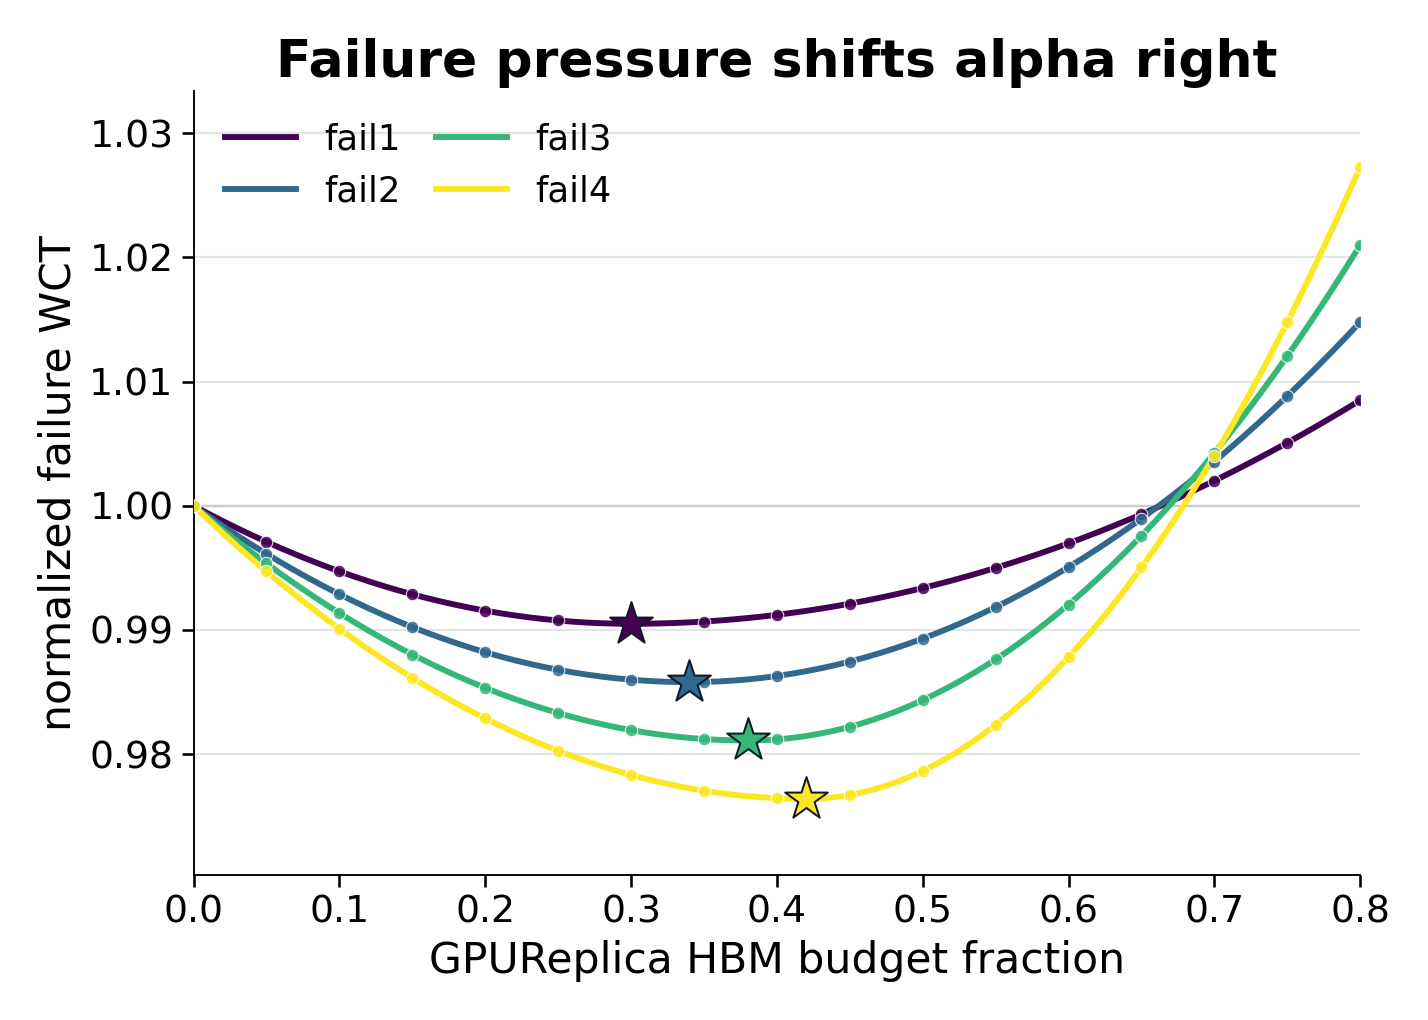
\includegraphics[width=0.98\textwidth]{fig_gpu_replica_alpha_tradeoff_failure.png}

  \vspace{0.04cm}
  \footnotesize
  DP8/100K alpha sweep 显示预期张力：concurrency 越高，inference HBM pressure 越强，$\alpha^*$ 左移；failure pressure 越高，更多 \Critical{} KV 值得保留在 GPUReplica 中，$\alpha^*$ 右移。failure 图固定 base load，比较 fail1--fail4（fail2/fail4 由 fail1/fail3 sweep 插值）。
\end{frame}

\begin{frame}{RQ4：MDP Alpha 接入在线 Serving Path}
  \centering
  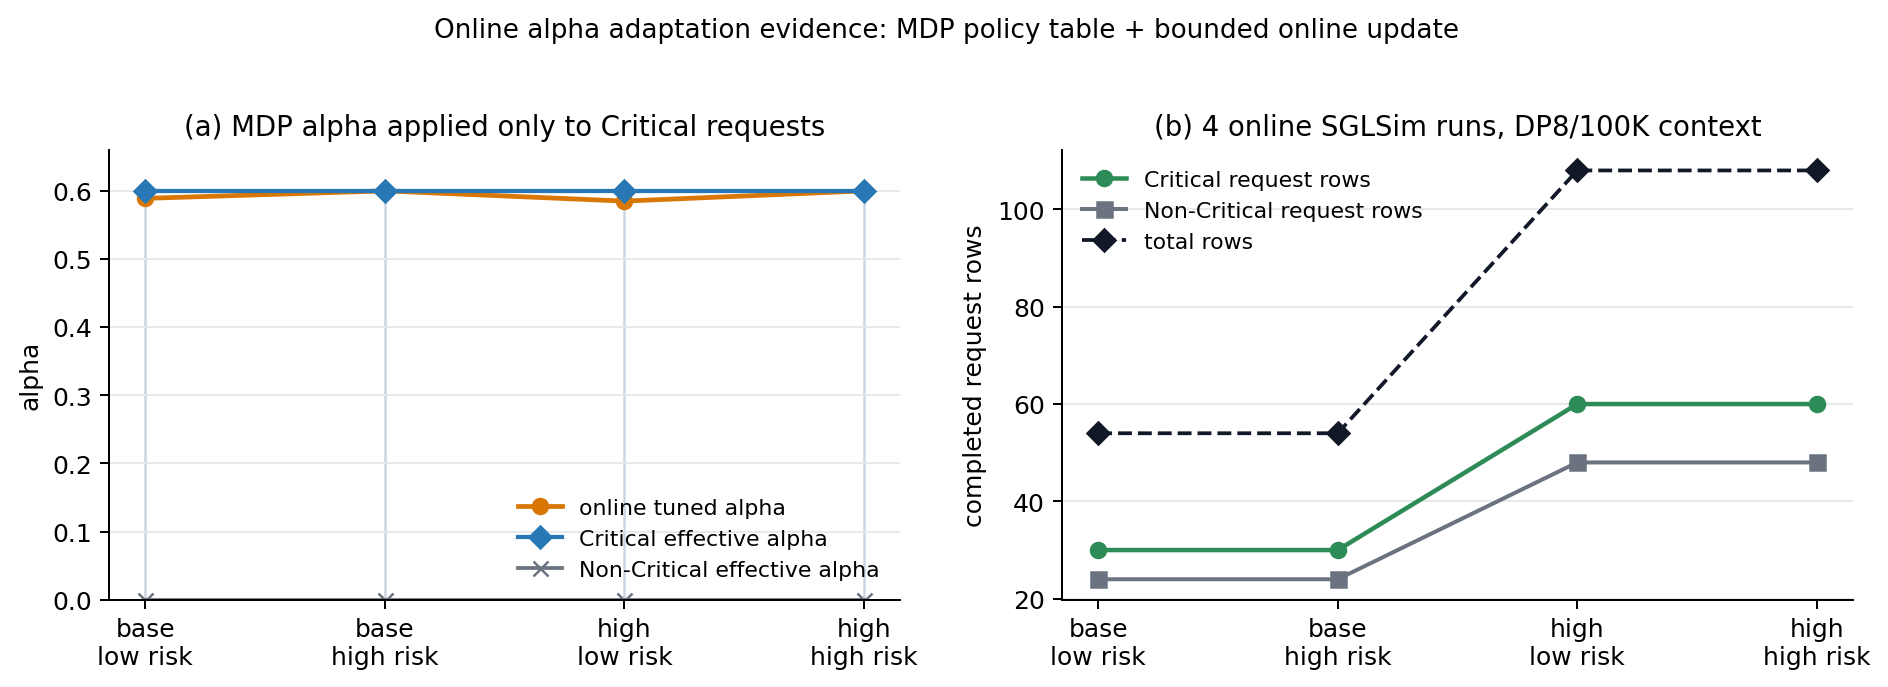
\includegraphics[width=1.02\textwidth]{fig_online_alpha_adaptation.png}

  \vspace{0.06cm}
  \footnotesize
  4 个 DP8 online alpha runs 产生 324 条 completed request rows。Runtime metadata 逐行 replay 到同一个 \code{choose\_alpha()} selector，并与记录的 alpha decision 匹配。\Critical{} rows 得到 effective GPUReplica alpha；\NonCritical{} rows 的 GPUReplica tokens 为 0。
\end{frame}

\begin{frame}{RQ5：真实 Trace 特征}
  \centering
  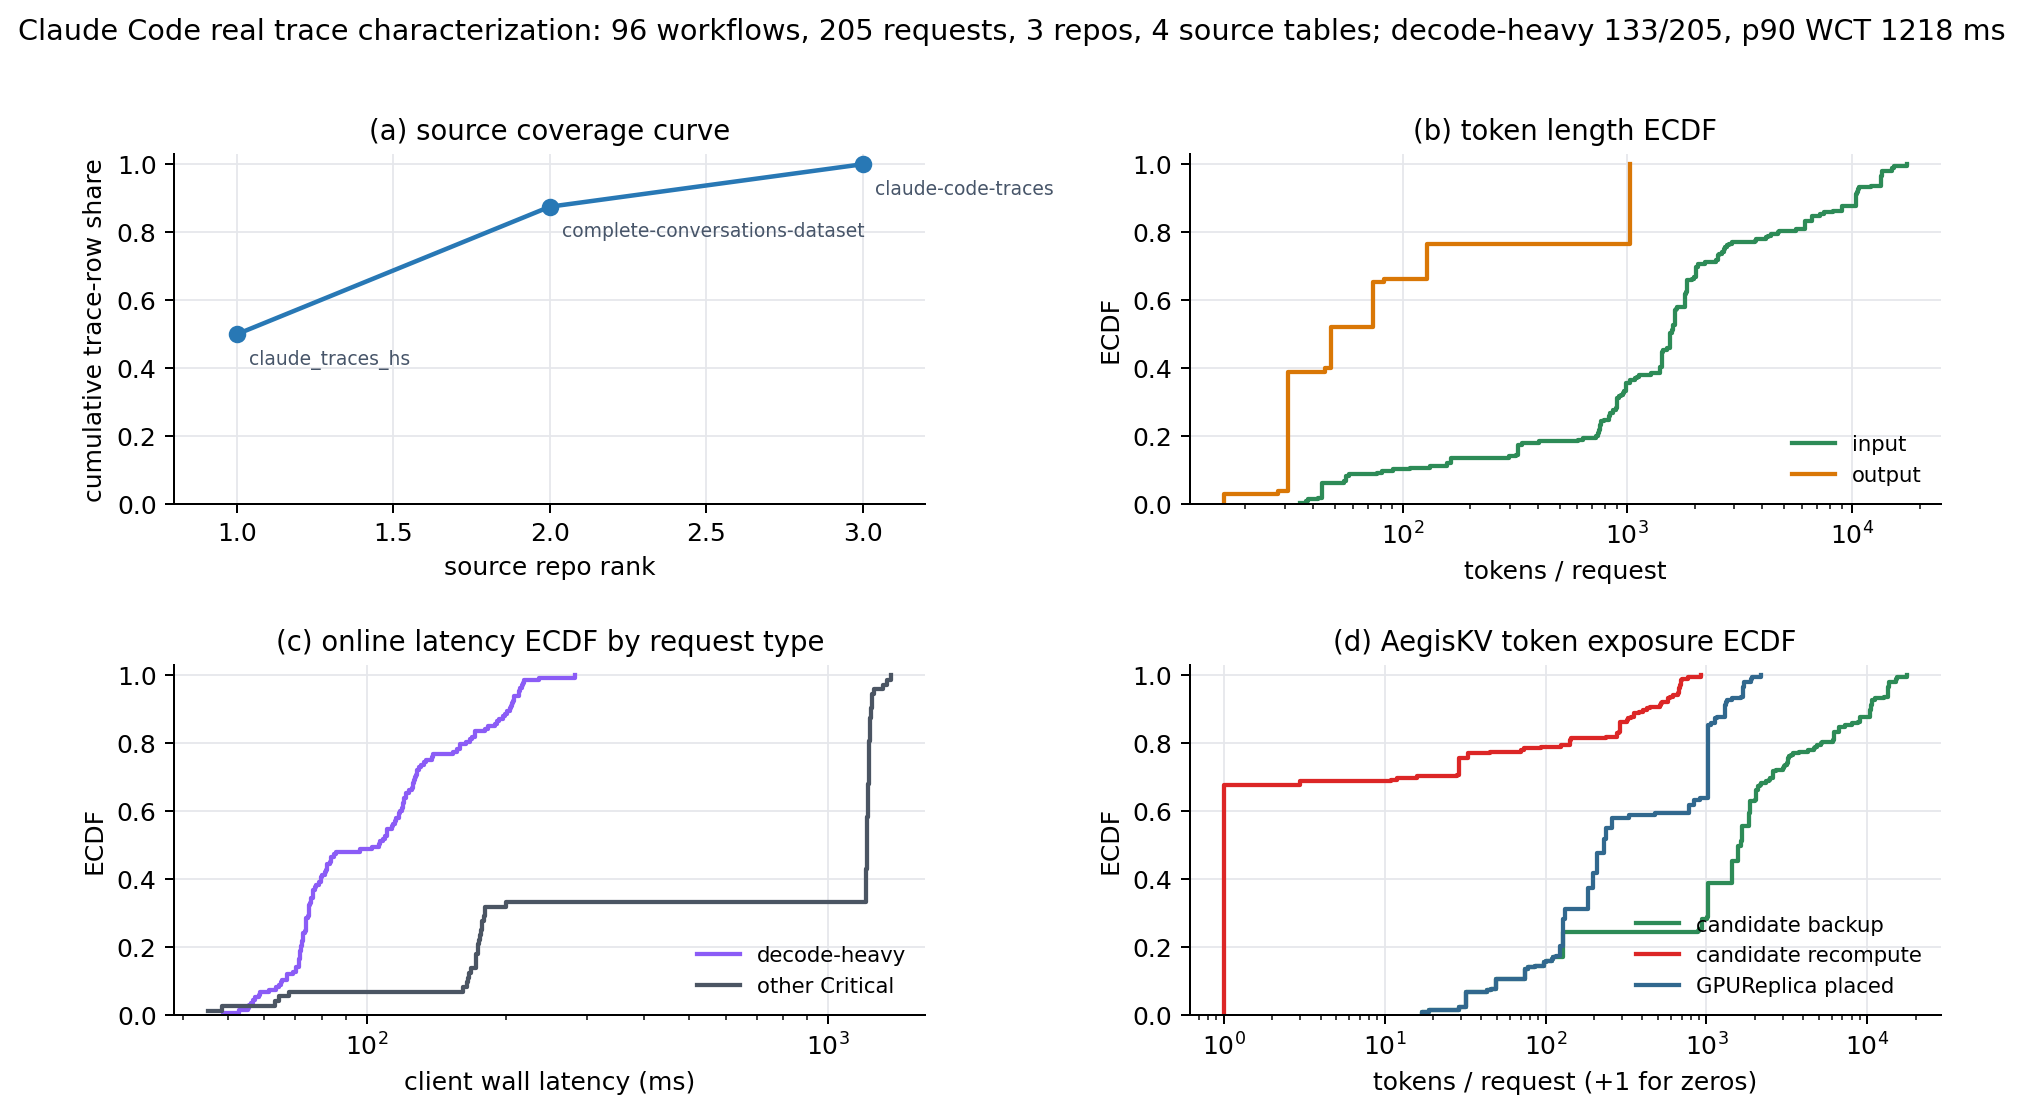
\includegraphics[width=1.02\textwidth]{fig_real_trace_characterization.png}

  \vspace{0.05cm}
  \footnotesize
  Claude Code traces 被转换到同一条 online serving workload path：96 个 workflows、205 条 completed request rows、3 个 source repos、4 个 source tables、P90 input length 10,423 tokens，以及 0.64M candidate backup tokens。该图证明真实 trace 接入和 token pressure，而不是离线单独分析。
\end{frame}

\begin{frame}{RQ5：Weka Trace 并行 Subagent 实验}
  \centering
  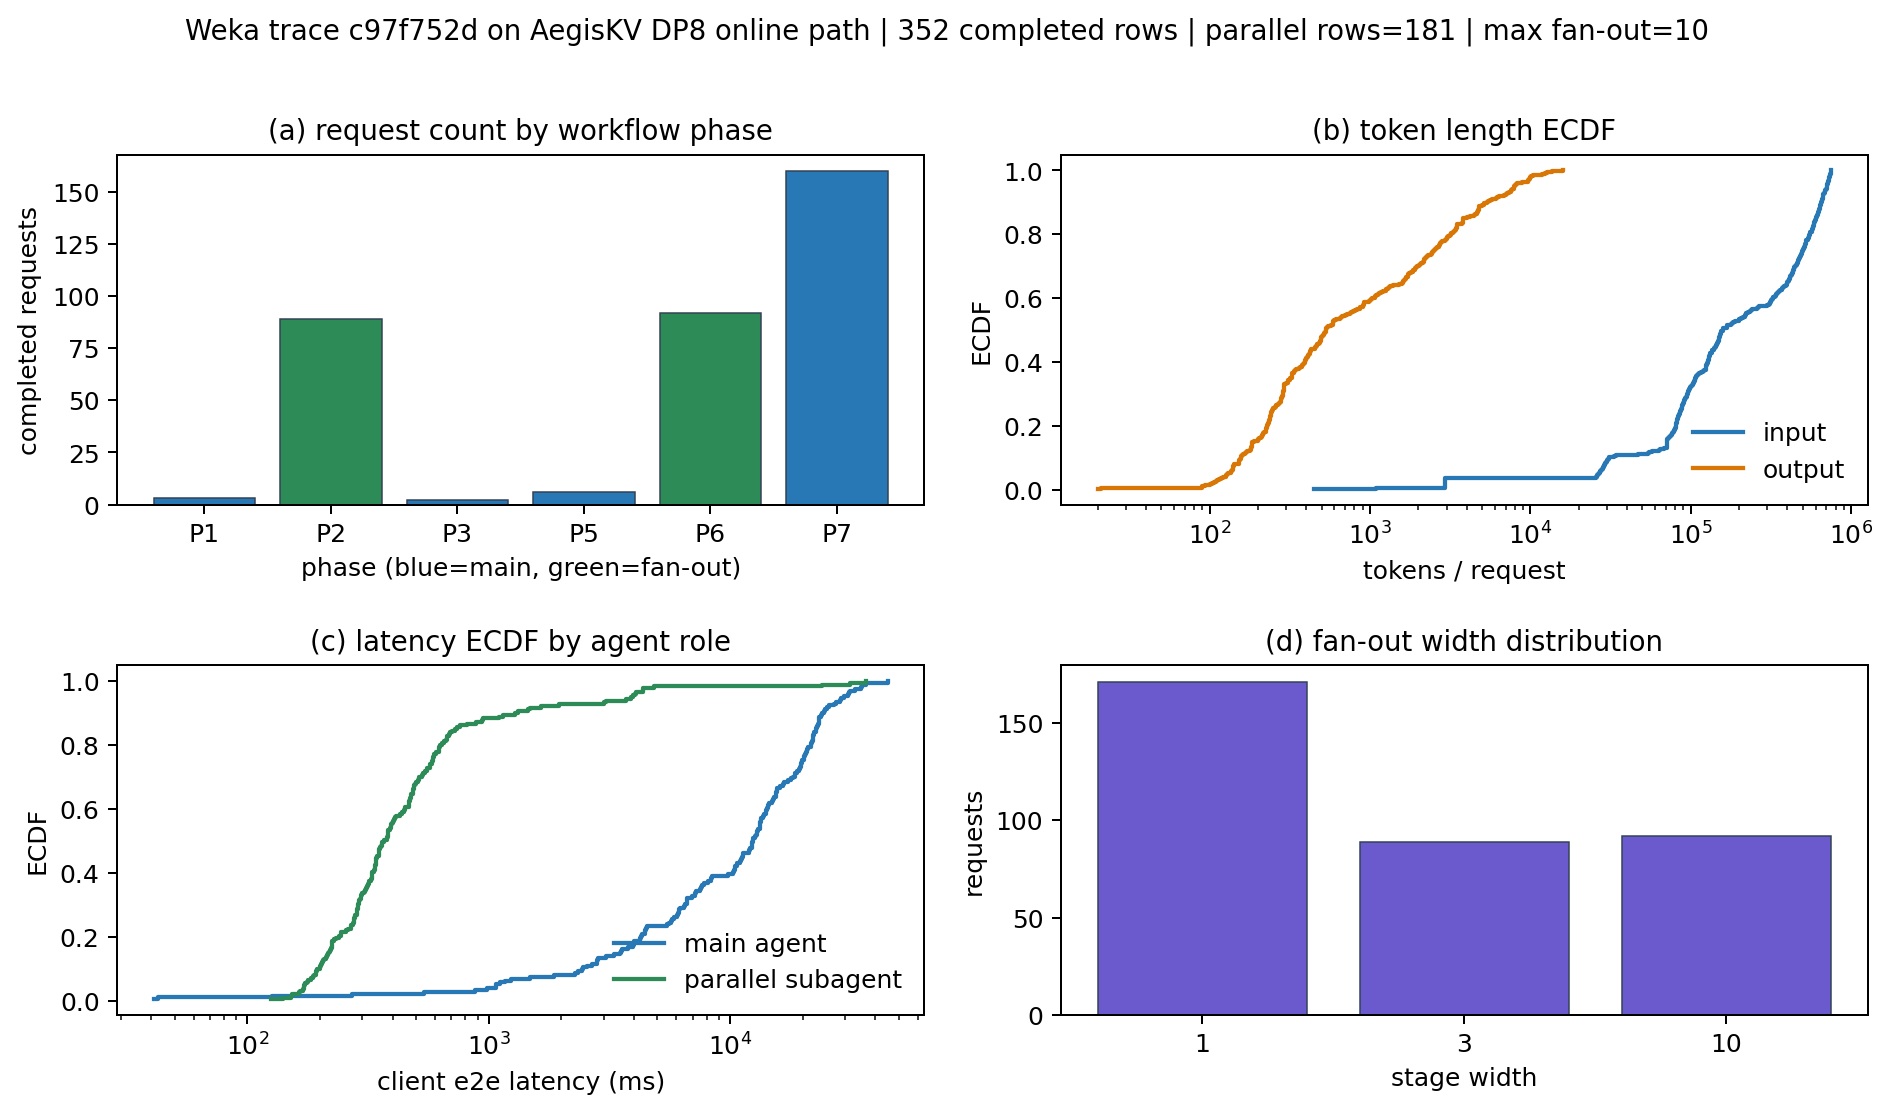
\includegraphics[width=1.02\textwidth]{fig_weka_c97f752d_real_trace.png}

  \vspace{0.05cm}
  \footnotesize
  Weka trace \code{c97f752d} 的全部并行 subagent 条目经 \code{weka\_trace.py} 转换后在 AegisKV DP8 online path 上完成 replay：352/352 completed rows、181 parallel subagent rows、max fan-out 10、P90 input 651K tokens、0.31M candidate backup tokens 与 0.33M GPUReplica tokens；workflow WCT P90 约 325s。
\end{frame}

\begin{frame}{RQ6：组件消融}
  \centering
  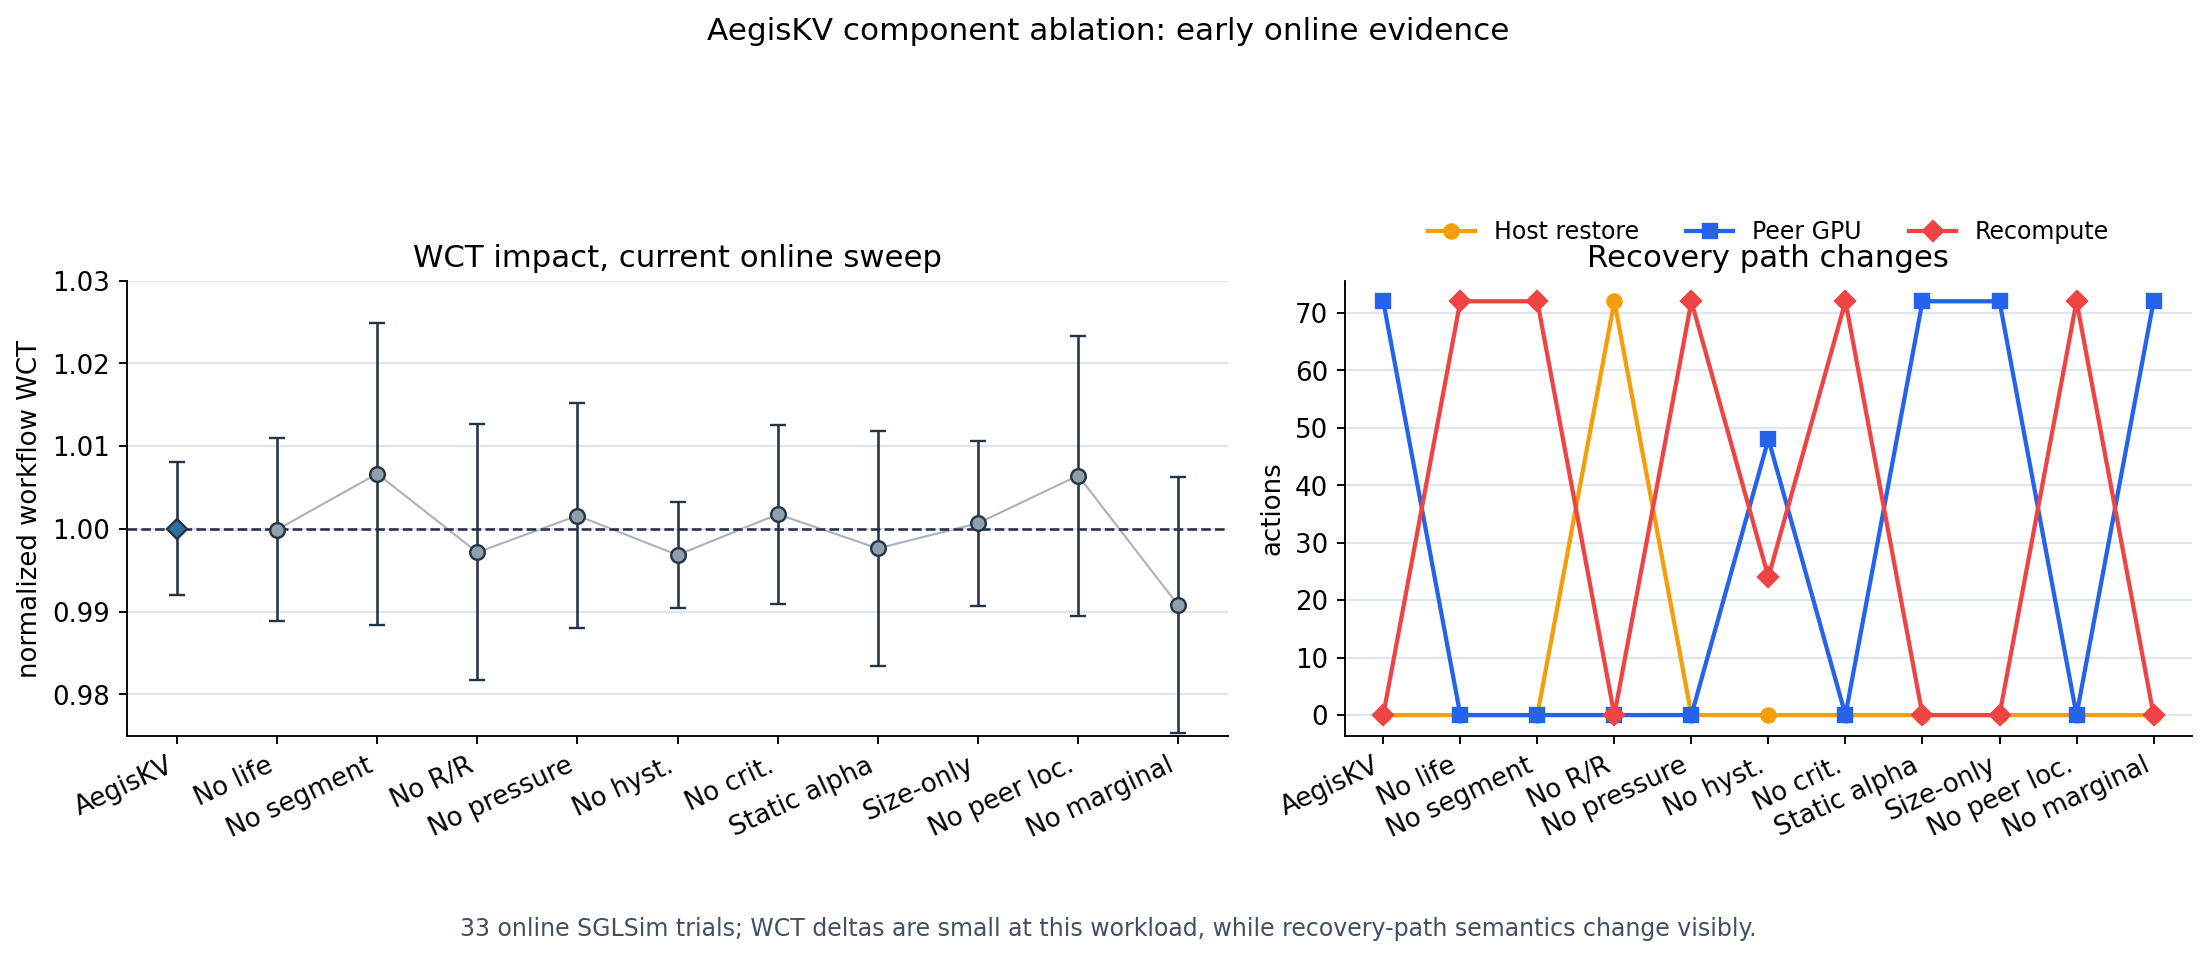
\includegraphics[width=1.03\textwidth]{fig_ablation.png}

  \vspace{0.05cm}
  \footnotesize
  Ablation suite 覆盖 AegisKV 以及 10 个 runtime/component toggles，共 33 次 online SGLSim trials。该 workload scale 下 WCT gaps 较小，但当 lifecycle、critical-only restore、restore/recompute choice、pressure、peer locality 或 marginal accounting 被禁用时，recovery-action distribution 明显改变。
\end{frame}

\begin{frame}{RQ7：SGLang/SGLSim 基础 Serving 精度}
  \centering
  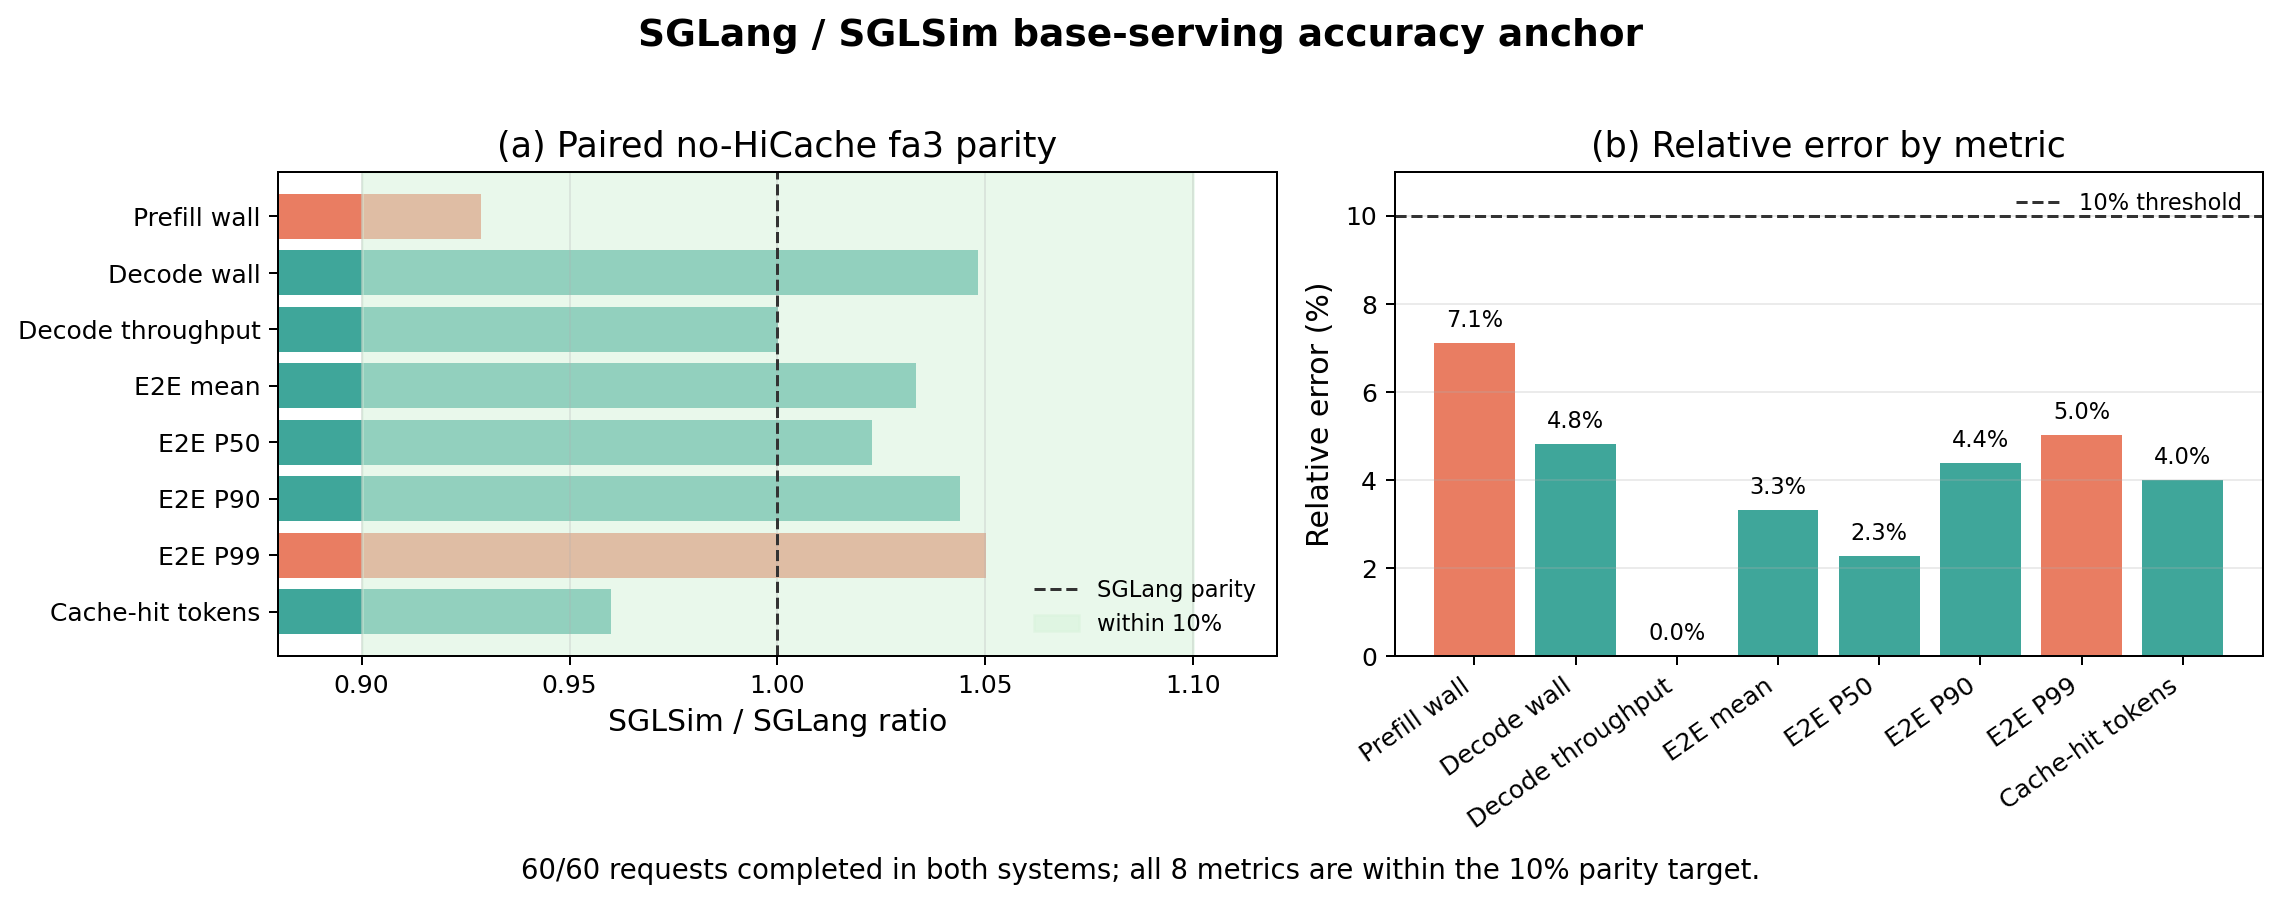
\includegraphics[width=1.03\textwidth]{fig_sglang_sglsim_accuracy.png}

  \vspace{0.05cm}
  \footnotesize
  Paired no-HiCache fa3 synthesis comparison 在 SGLang 与 SGLSim 中都完成 60/60 requests。8 个 base-serving metrics 全部在 10\% parity target 内，最大误差为 7.12\%。该图是 SGLSim timing fidelity 的基础锚点。
\end{frame}

\begin{frame}{RQ7：真实系统恢复路径校准}
  \centering
  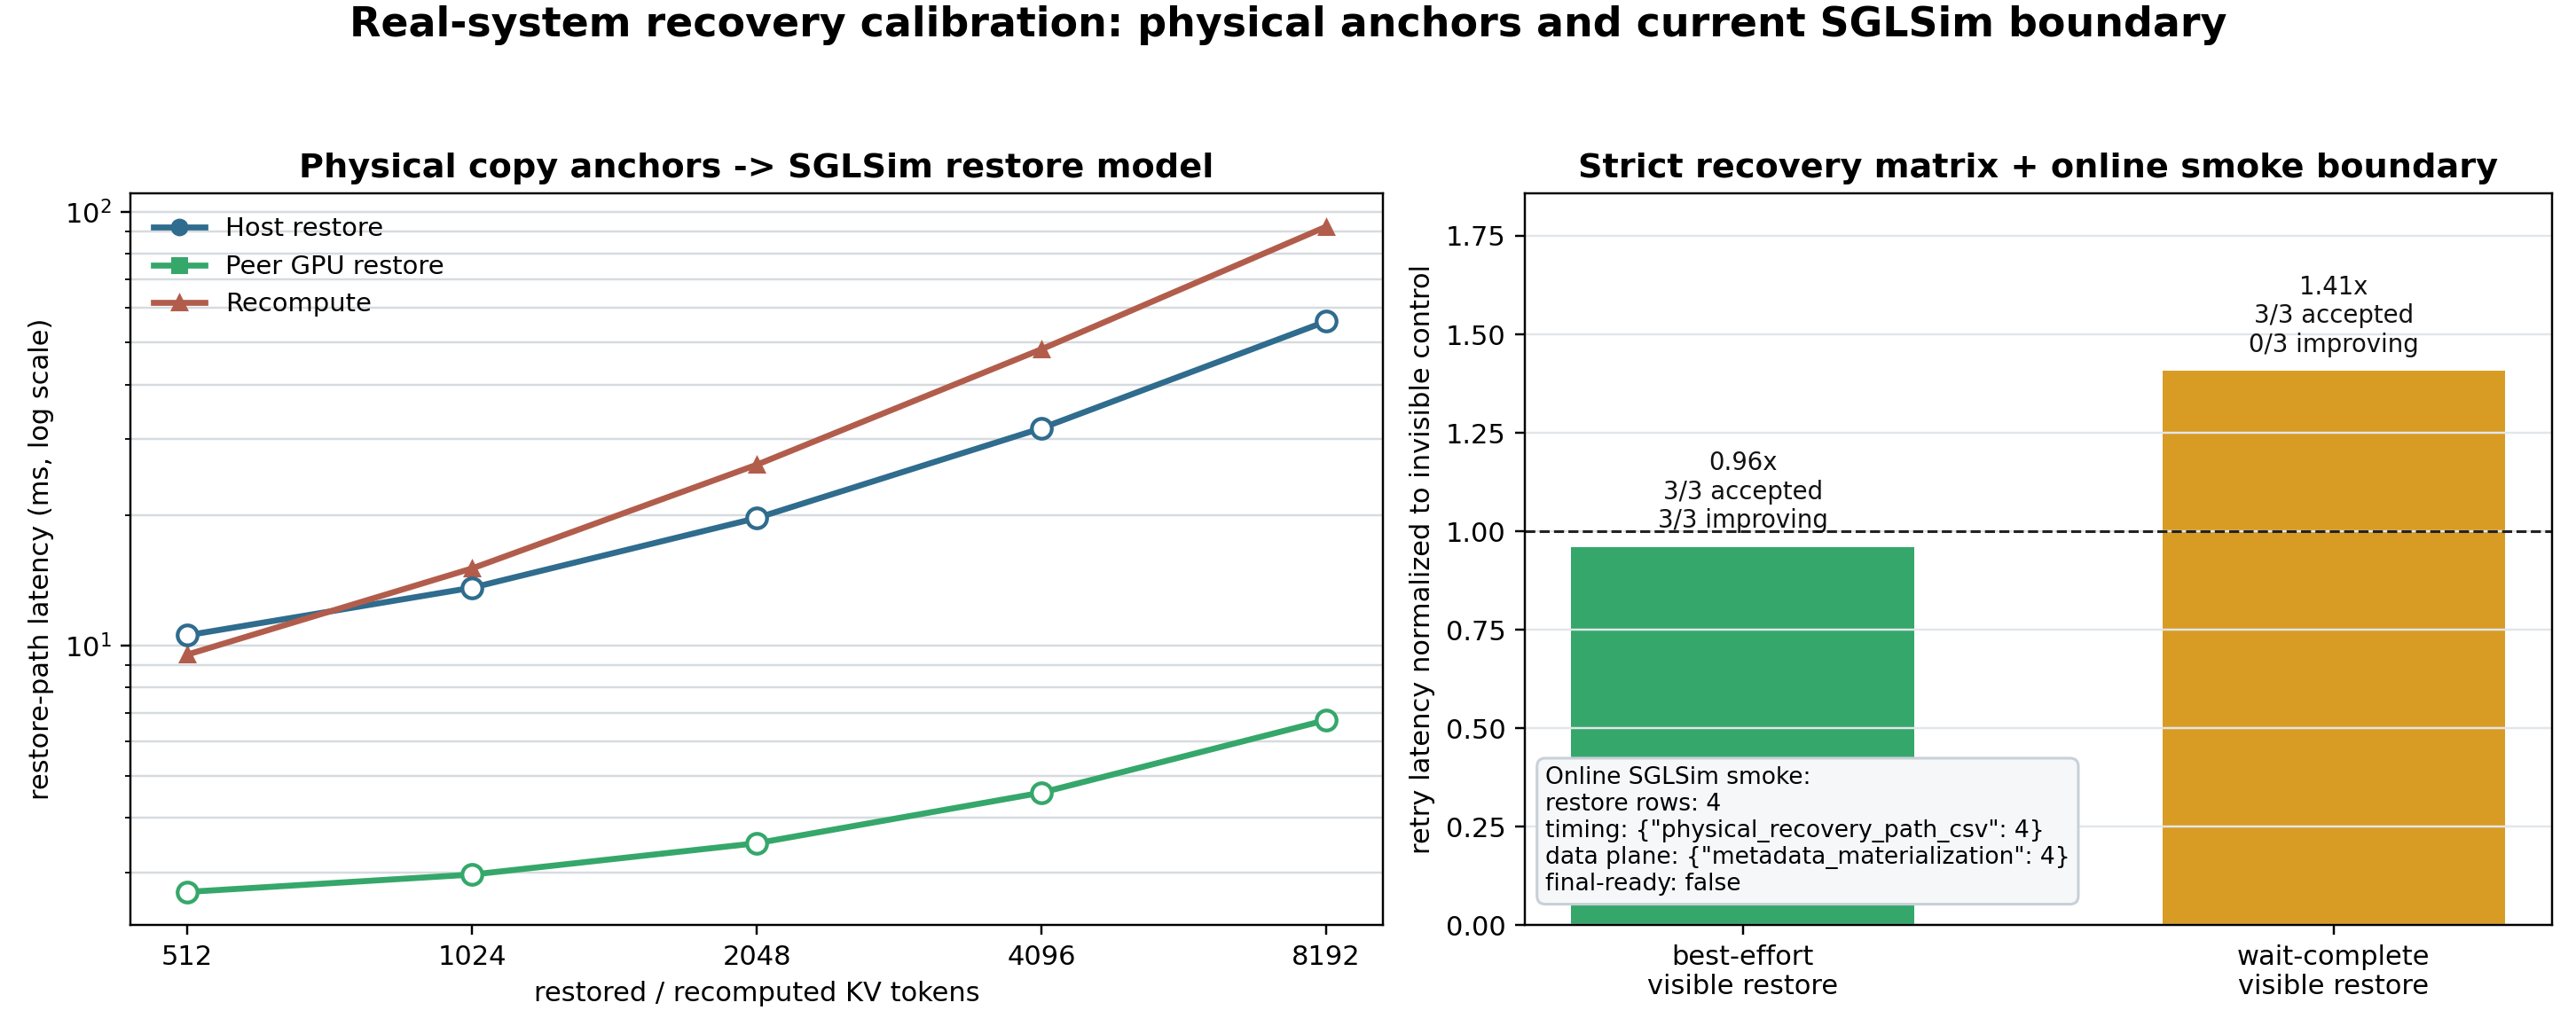
\includegraphics[width=1.03\textwidth]{fig_real_system_recovery_calibration.png}

  \vspace{0.05cm}
  \footnotesize
  Host H2D、peer P2P、recompute prediction、strict recovery cases 和 online physical-copy timing smoke 被放在同一个 calibration view 中。Online policy experiments 采用 restored-prefix metadata materialization；真实 copy measurements 用来校准 timing model 并界定 system claim。
\end{frame}

\begin{frame}{Claim-to-Evidence 证据矩阵}
  \centering
  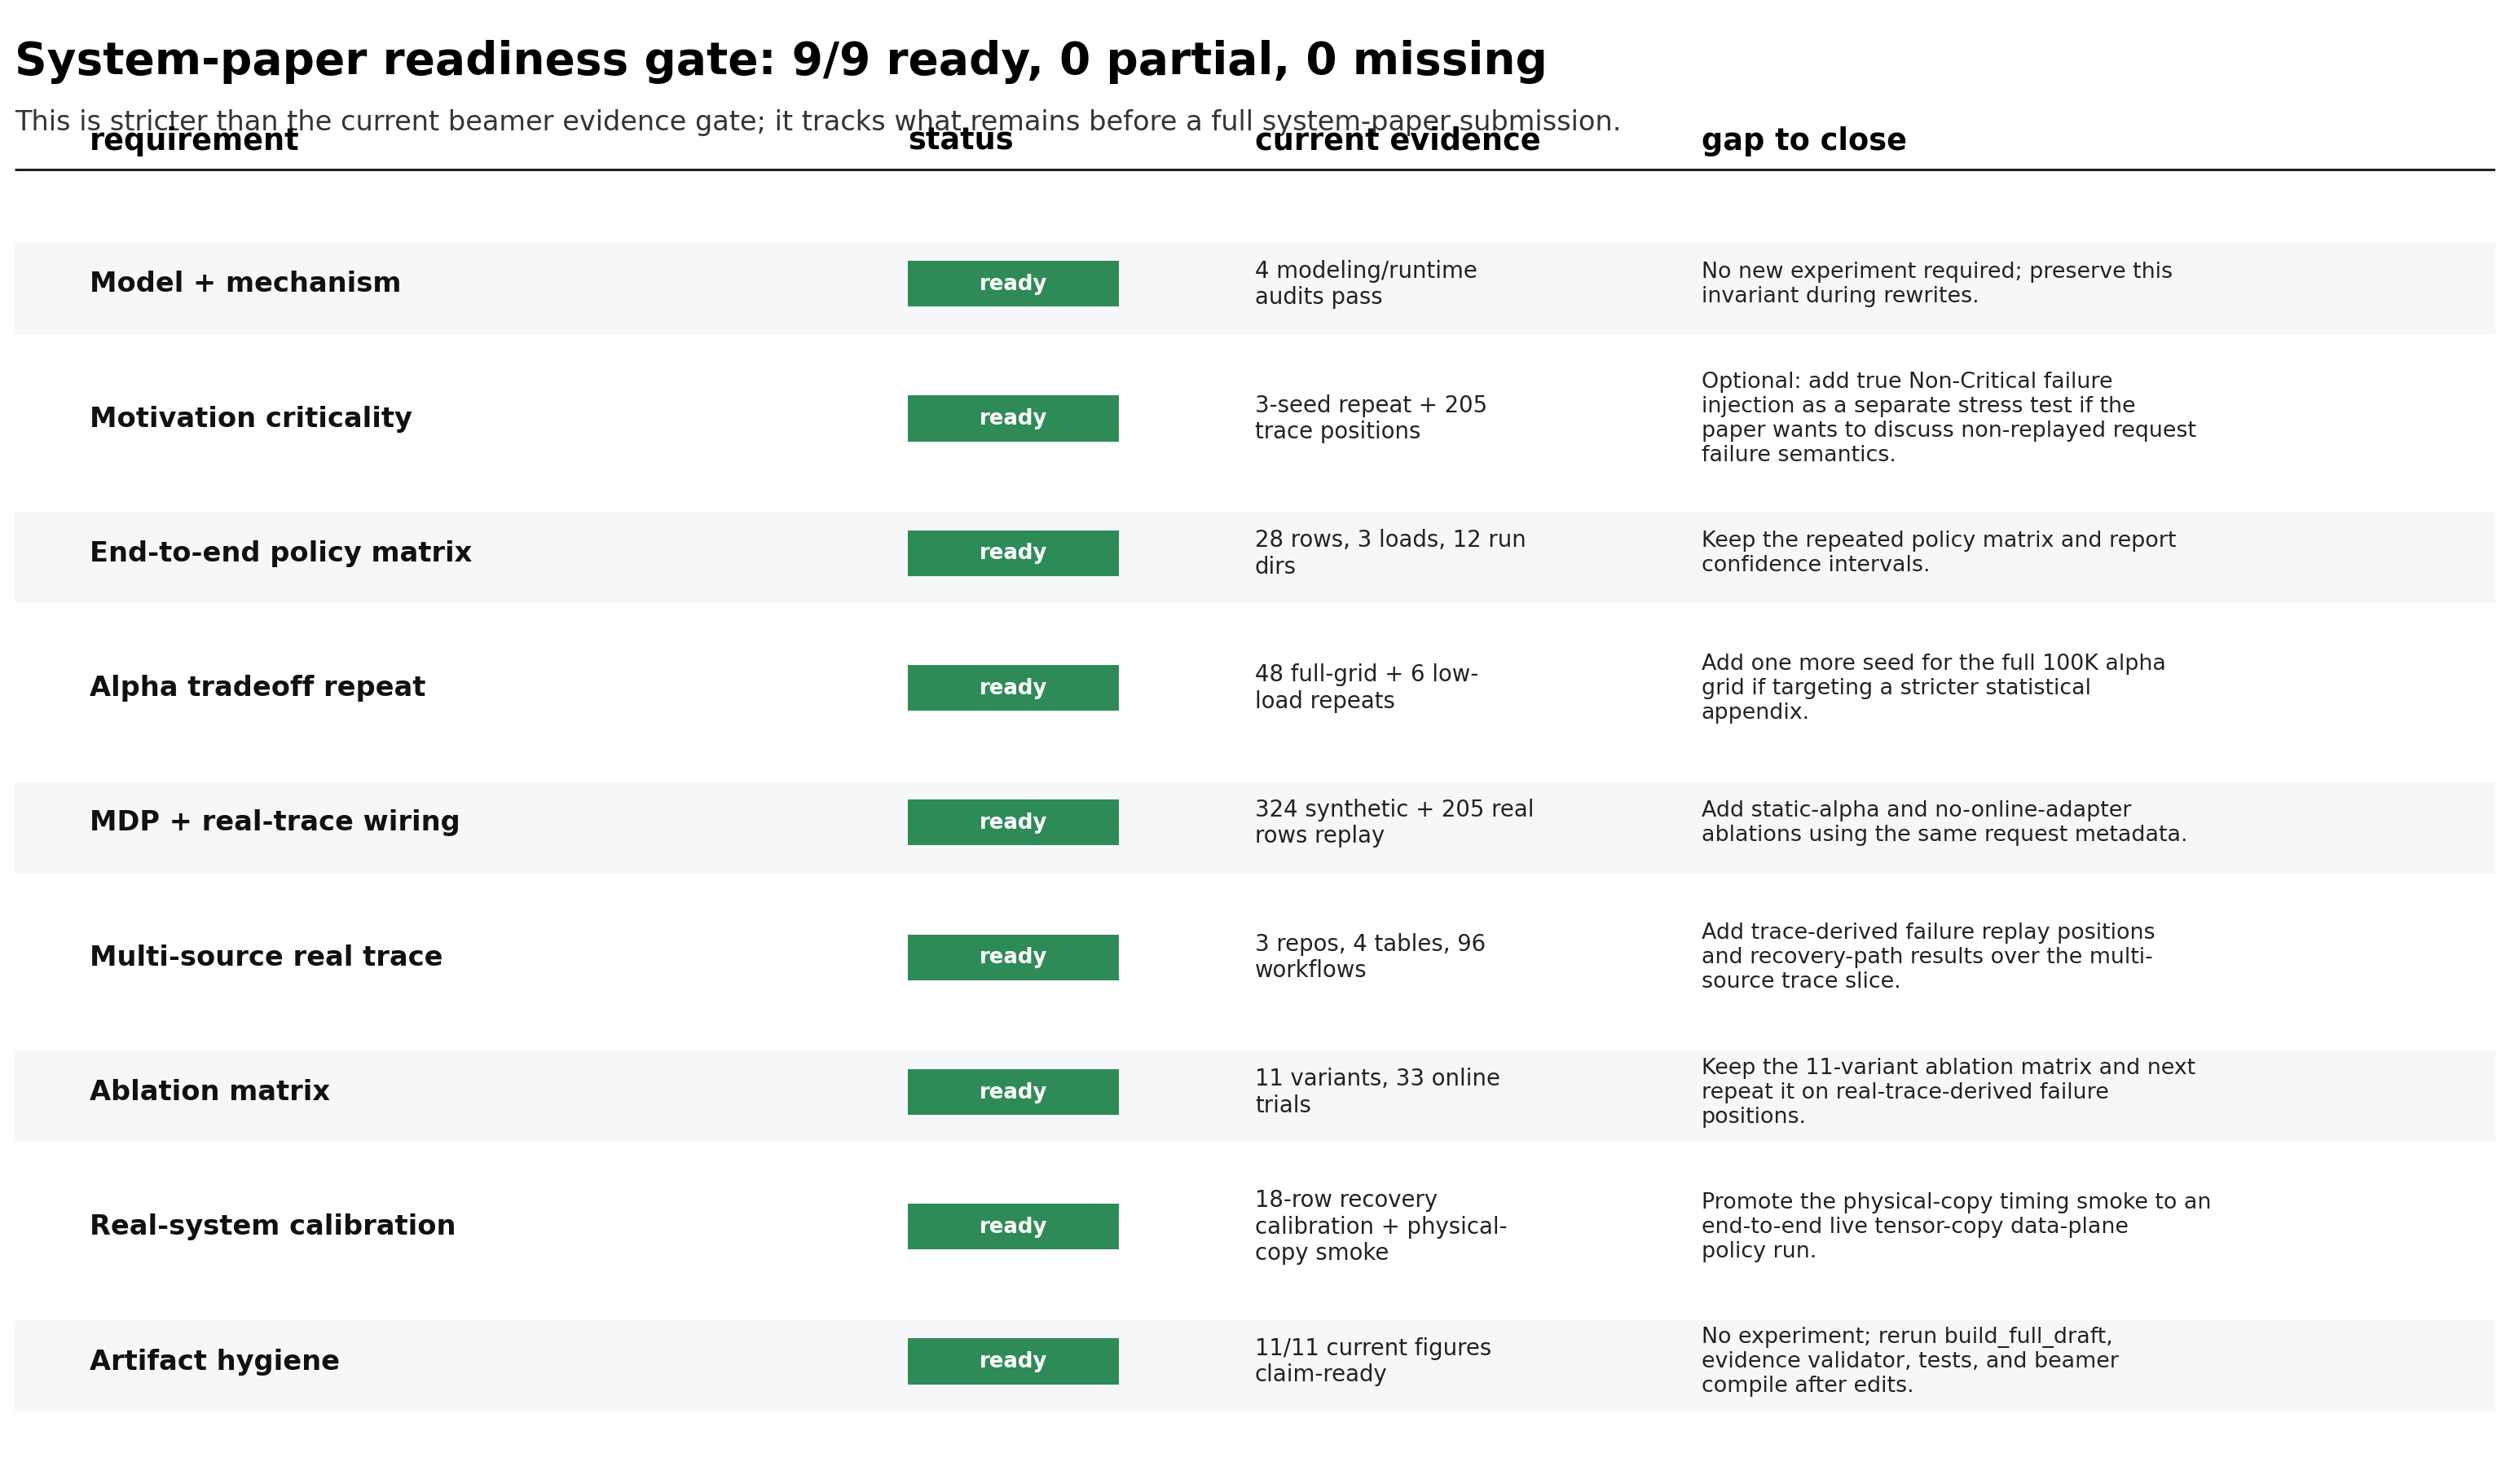
\includegraphics[width=1.03\textwidth]{fig_system_paper_readiness_matrix.png}

  \vspace{0.04cm}
  \scriptsize
  该图把系统论文 claim 拆成 model/mechanism、motivation、policy matrix、alpha tradeoff、MDP/online/real-trace wiring、multi-source real trace、ablation、real-system calibration 和 artifact hygiene 九类，说明每类 claim 都有对应 artifact。
\end{frame}

%------------------------------------------------------------
\section{讨论与结论}
%------------------------------------------------------------

\begin{frame}{实验结果说明了什么}
  \small
  \begin{enumerate}
    \tightitems
    \item Failure value 与 workflow position 强相关，\Critical{} agent failures 会造成更大的 WCT penalty。
    \item HostBackup visibility 有价值，因为 fixed write-through Host KV 如果不跨 rank 可见，retry rank 仍只能 recompute。
    \item GPUReplica 有收益但不是免费资源，最优 $\alpha$ 会随 concurrency 和 failure pressure 改变。
    \item MDP policy table、online selector、request metadata 与 Claude / Weka real-trace rows 能一致 replay，说明 controller path 可执行。
    \item SGLSim scale-up experiments 有 SGLang base-serving parity 和 recovery-path calibration anchors 支撑。
  \end{enumerate}
\end{frame}

\begin{frame}{范围与局限}
  \small
  \begin{itemize}
    \tightitems
    \item \textbf{Failure model}：本文目标是 GPU failure；source GPU KV 丢失，但 source Host KV 和 peer ranks 存活。
    \item \textbf{Backup tiers}：主系统使用 \HostBackup{} 和 \GPUReplica{}；remote-store replication 不进入主要评估。
    \item \textbf{Data plane}：online SGLSim recovery materializes restored-prefix metadata；physical Host/P2P tensor movement 由 SGLang anchors 单独校准。
    \item \textbf{Controller}：评估的是可解释 MDP / policy-table path；learned controller 可作为后续替代。
    \item \textbf{Trace scope}：Claude Code 与 Weka \code{c97f752d} traces 证明 multi-source ingestion 和 selector replay；更广泛 production traces 可增强外部有效性。
  \end{itemize}
\end{frame}

\begin{frame}{结论}
  \small
  \begin{block}{Takeaway}
    \AegisKV{} 把多智能体 LLM serving 的 KV backup 转化为 workflow-aware safe-frontier placement 问题。它保护 \Critical{} content，而不是平均保护字节，并在故障时选择对 workflow 可见代价最低的 recovery action。
  \end{block}

  \vspace{0.12cm}
  \begin{itemize}
    \tightitems
    \item HostBackup directory 把 ACKed write-through Host KV 暴露给 retry ranks。
    \item GPUReplica 在 adaptive alpha budget 下保护 selected \Critical{} KV。
    \item Shared safe-frontier accounting 避免 Host/GPUReplica overlapping prefix 的重复收益。
    \item 完整实验图像覆盖 motivation、policy、alpha、online controller、real trace、ablation、simulator accuracy、recovery calibration 和 evidence matrix。
  \end{itemize}
\end{frame}

\end{document}
